% !TEX program = xelatex
% 编译：TEXINPUTS=.: xelatex main.tex（运行两次）
\documentclass[12pt,a4paper]{article}
\usepackage[top=2.6cm,bottom=2.6cm,left=2.25cm,right=2.25cm,footskip=1.2cm]{geometry}
\usepackage{amsmath,amssymb,amsthm}
\usepackage{unicode-math}
\setmainfont{TeX Gyre Termes}
\setsansfont{TeX Gyre Termes}
\setmathfont{TeX Gyre Termes Math}
\usepackage{xeCJK}
\setCJKmainfont[BoldFont={Noto Sans CJK SC Bold},ItalicFont={Noto Sans CJK SC}]{Noto Serif CJK SC}
\setCJKsansfont[BoldFont={Noto Sans CJK SC Bold}]{Noto Sans CJK SC}
\setCJKmonofont{Noto Sans Mono CJK SC}
\newCJKfontfamily\heiti[BoldFont={Noto Sans CJK SC Bold}]{Noto Sans CJK SC}
\newCJKfontfamily\heitibf{Noto Sans CJK SC Bold}
\xeCJKsetup{CJKecglue={\hskip 0.15em plus 0.05em}}
\usepackage{graphicx,float,booktabs,array,multirow,makecell,tabularx,longtable}
\usepackage{caption,subcaption}
\usepackage{titlesec,enumitem,indentfirst,xcolor,listings,pdfpages,fancyhdr}
\usepackage[normalem]{ulem}
\usepackage[hidelinks]{hyperref}
\graphicspath{{figs/}}

% ---------- 版式 ----------
\linespread{1.18}\selectfont
\setlength{\parindent}{2em}
\setlength{\parskip}{1pt plus 1pt}
\pagestyle{plain}
\renewcommand{\figurename}{图}
\renewcommand{\tablename}{表}
\renewcommand{\refname}{参考文献}
\captionsetup{labelsep=quad,font=small,skip=4pt}
\captionsetup[table]{position=top}
\setlist{nosep,leftmargin=2.2em}

\titleformat{\section}{\centering\large\heiti}{\thesection}{1em}{}
\titleformat{\subsection}{\normalsize\heitibf}{\thesubsection}{1em}{}
\titleformat{\subsubsection}{\normalsize\heiti}{\thesubsubsection}{1em}{}
\titlespacing*{\section}{0pt}{12pt}{8pt}
\titlespacing*{\subsection}{0pt}{8pt}{4pt}
\titlespacing*{\subsubsection}{0pt}{6pt}{3pt}

\theoremstyle{plain}
\newtheorem{proposition}{命题}
\theoremstyle{definition}
\newtheorem{definition}{定义}

\newcommand{\bp}{\symbf{p}}
\newcommand{\dex}{\,\mathrm{dex}}

\lstset{basicstyle=\ttfamily\small,frame=single,framesep=4pt,columns=fullflexible,
  keepspaces=true,breaklines=true,showstringspaces=false,
  keywordstyle=\bfseries,language=Python,xleftmargin=4pt,xrightmargin=4pt}

\begin{document}

% ================= 封面（第 0 页，直接取自官方格式模板） =================
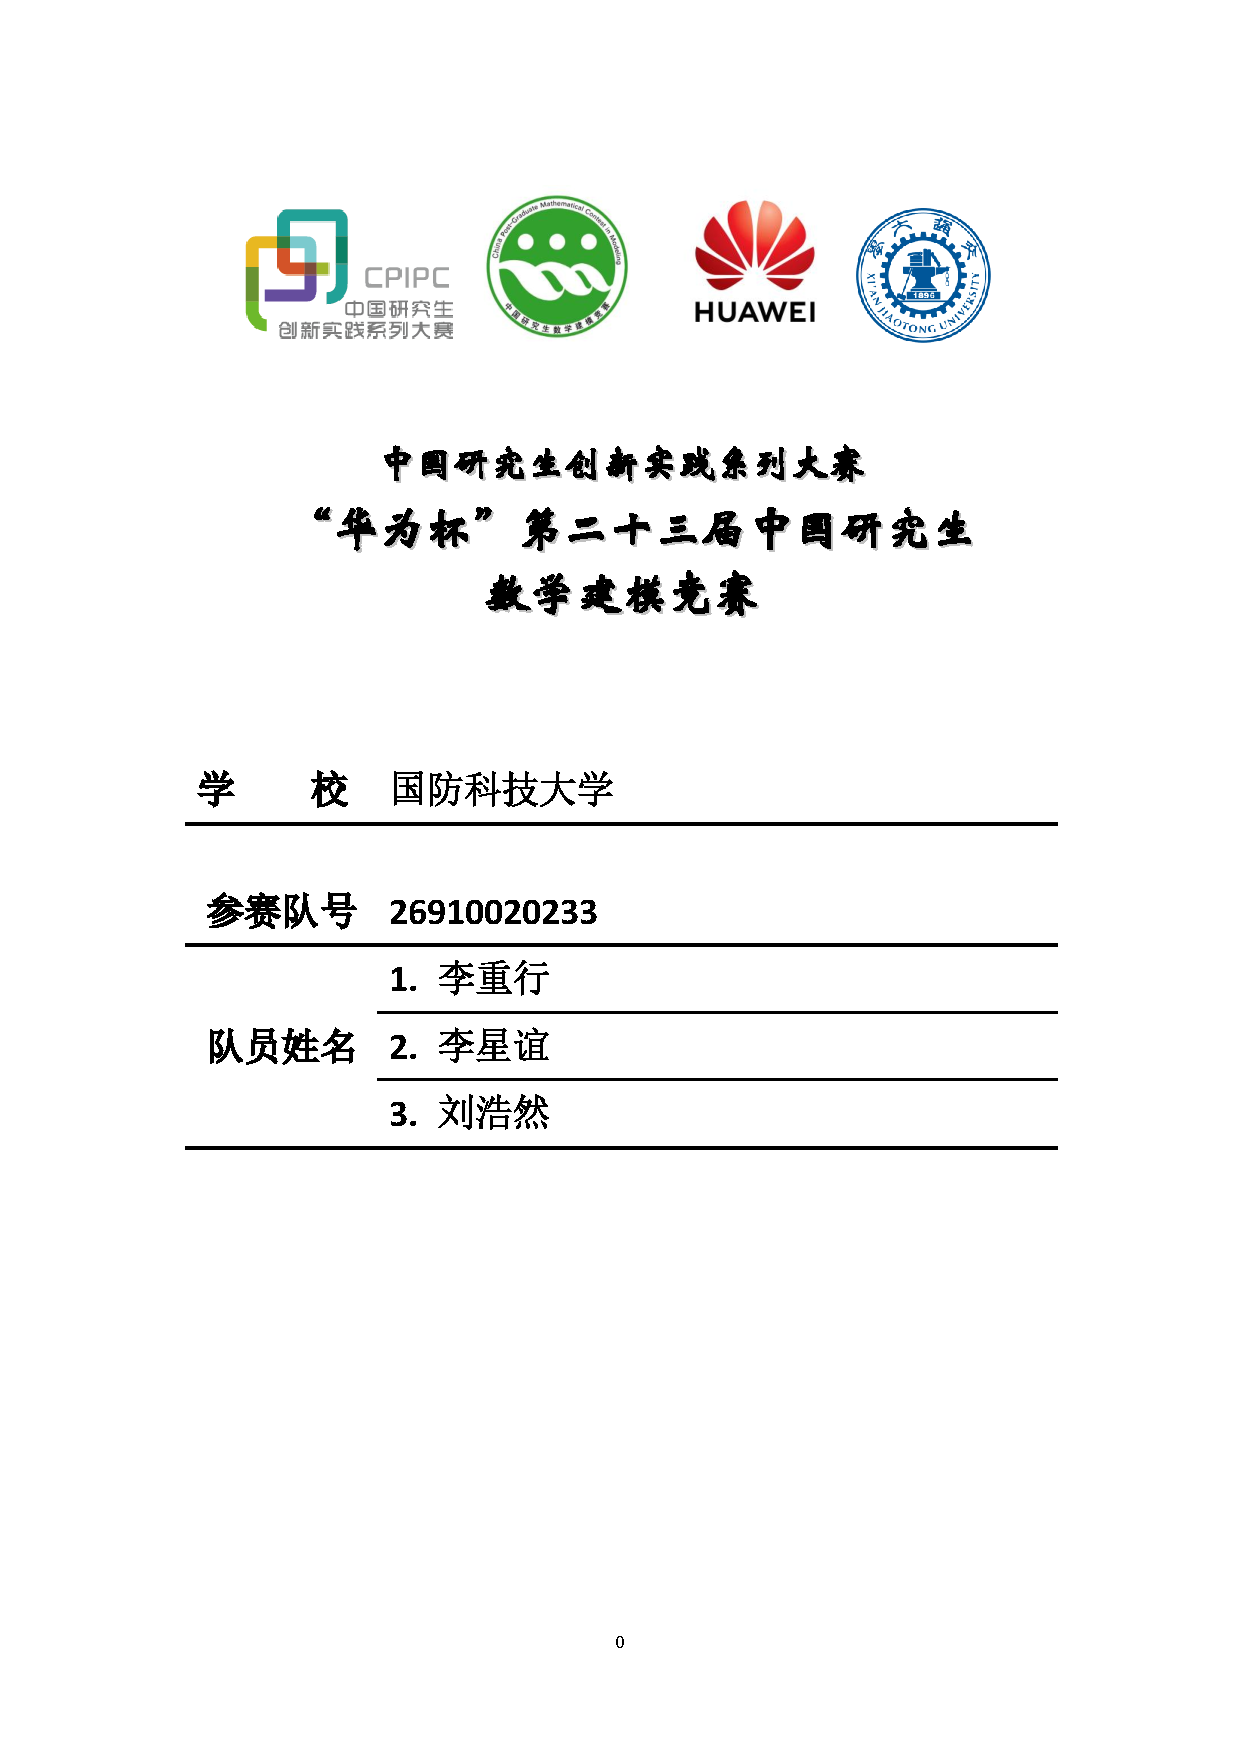
\includepdf[pages=1]{format_template.pdf}
\setcounter{page}{1}

% ================= 标题与摘要页 =================
\begin{center}
\vspace*{0.6cm}
{\heitibf\fontsize{18pt}{24pt}\selectfont 中国研究生创新实践系列大赛}\\[6pt]
{\heitibf\fontsize{22pt}{28pt}\selectfont “华为杯”第二十三届中国研究生}\\[6pt]
{\heitibf\fontsize{22pt}{28pt}\selectfont 数学建模竞赛}
\end{center}
\vspace{0.9cm}
\noindent{\heiti\large 题\quad 目：}\hfill
\uline{\makebox[0.78\textwidth][c]{\large 算力约束下提升大语言模型能力的资源配置建模}}
\vspace{0.9cm}
\begin{center}{\heitibf\Large 摘\quad 要：}\end{center}
\vspace{0.1cm}

大语言模型的能力由参数规模 $N$、数据量 $D$、数据质量 $Q$ 与领域配比 $\bp$ 共同决定，而扩大规模、提升质量与延长上下文都要消耗有限的算力。本文沿赛题“数据刻画—规律建模—资源优化—演进预测”的递进主线建立四个模型，以接口文件组织各问结果，并按证据等级（来源观测、半合成、外推估算）区分各附件的用途。

针对问题一，将 22 个质量字段展开为 25 个方向统一的指标，以 CRITIC 权重和加权 Huber 中心构造样本级主质量分 $Q$，并取中位数聚合为领域质量分。A1 与对应全量扩展集 A2/A3 的分布未检出显著差异（KS 检验 $p=0.313/0.220$）。评分后以六个来源定义高分歧候选；A1/A2/A3 的候选比例为 $5.00\%/4.73\%/4.99\%$，多来源对立候选比例为 $1.36\%/1.58\%/1.77\%$。基于 A16/A18 将七个质量领域桥接到 17 个配比领域，并用 clr 回归建立配比与 13 个验证域交叉熵的定量关系；1M 留出集的平均逐域 $R^2=0.772$。GBDT 搜索得到的等权候选配比相对均匀配比预测降损 $9.915\%$。冻结 1M 模型在 60M/1B 留出集的配比排序 Spearman 为 $0.467/0.677$，但绝对损失预测不具跨尺度可迁移性；A12--A15 为估算/外推数据，仅用于边界讨论。

针对问题二，先以 B1 校准经典标度律，再用 B2、B4、B5 检查跨来源趋势。固定经典基线后，在 B6 拟合广义质量项 $L=L_0+(1-Q_B)(\kappa_NAN^{-\alpha}+\kappa_DBD^{-\beta}+k_0)$，并在 B7 新增 90 个半合成点上留出检验（RMSE $0.042$）；B8 的质量方向与 B6/B7 不一致，不并入拟合。A、B 之间的映射在聚合可加及 B 侧惩罚仿射等假设下可推出为仿射，但锚点仍是建模选择；配比组成修正尚未标定。该半合成模型给出质量弹性、质量地板、质量—规模替代条件及算力最优规模的解析式，结论不等同于真实训练规律。

针对问题三，三项成本都与 $D$ 成正比，最优时预算约束必取等，据此把 $D$ 解析消去，将问题化为 $(\log N,Q)$ 上的二维无约束问题，并用“内层黄金分割 + 外层三级网格加密”的向量化求解器，在 3 种成本函数 × 7 档预算 × 5 档 $L_{\mathrm{ctx}}$ × 2 种基线质量下求得 210 组最优解。数值解与闭式解的相对误差不超过 $1.83\times10^{-7}$，与穷举网格的 Loss 差不超过 $1.6\times10^{-5}$。以 KKT 活跃约束集的改变定义结构性转移，并由边际比 $\Phi(C)=1$ 解析识别临界预算。旧接口主口径（$Q_0=0.988$，$L_{\mathrm{ctx}}=2048$）下，$\log_{10}C_{\mathrm{crit}}$ 为：指数型 $20.61$、幂函数型 $20.48$、对数型 $18.52$。三种识别口径的极差不超过 $0.05\dex$，bootstrap 90\% 区间在 $\pm0.03\dex$ 以内。转移几乎呈“不提质 → 提满”的跳变，210 组中 34 组为 $Q_0$ 角点、3 组为内点，均出现在 $10^{19}$–$10^{20}$。解析给出 $L_{\mathrm{ctx}}^{\mathrm{crit}}=6/\eta=30000$；上下文增至 131k 时，$C=10^{22}$ 的最优模型缩至 $0.48$ 倍，注意力成本占 $81\%$。将配比联立优化可再降 $13.7\%$，但几乎全部来自配比效应；最优配比排序在不同预算下的秩相关 $\ge0.976$，“先定配比、再定规模”的分离策略成立。

针对问题四，能力的主口径为 C1 的 Average，并对 C8 的 39 个叶子任务逐一聚合，识别出 10 个饱和任务，构造去饱和综合分，发现饱和任务使前沿增速被低估约 1.6 倍。将 base 与 chat 分开处理，时间轴采用 C2 发布日。按可比性等级分层，用加权 sigmoid 拟合 C6 的 Loss–Benchmark 桥接（$r=-0.51$，留一 RMSE $8.08$，优于线性的 $8.28$）。以问题二的标度律 $\hat L(N,D)$ 作为规模状态，建立“S 形桥接 + 时间技术项”的结构模型（$R^2=0.87$），并用 Shapley 分解前沿增长。2023.5→2025.0 期间 base 前沿由 $12.5$ 升至 $37.3$，结构口径下非规模技术进步占 $13\%$–$23\%$，线性效率前沿口径为 $38\%$–$46\%$；两类方法的差异来自对 S 形加速段的归因不同。结论是规模扩张占主导。预测以问题三的最优配置为算力通道，在基线 / 减半 / 1/4 三种算力增速（$0.60/0.30/0.15\dex/\mathrm{yr}$）情景下，base 开源前沿 24 个月中位数为 $46.2/45.2/44.1$。算力放缓时，技术进步在增量中的占比由 $55\%$ 升至 $77\%$。回测误差为 $-0.78$，而朴素线性外推为 $+2.65$。

问题二的质量形式与问题一当前质量接口尚未贯通，问题三、四的上述数值仍基于旧的 $Q$ 锚点和旧标度律接口；在新接口下完成重估前，这些下游数值不应解读为修订模型的预测结果。

各问按数据结构分别采用留出检验、跨来源趋势对照或解析—数值核查，《数据说明》中的“建议”也逐条核对。B6/B7 的新质量项目前报告点估计与半合成留出结果，未完成可复现的区间估计；问题三、四仍使用旧接口，需贯通重算后再解释为修订模型下的结论。半合成与外推数据只支持其明确标注的形式与边界讨论。

\vspace{6pt}
\noindent{\heitibf 关键词：}CRITIC 赋权；成分数据 clr 回归；广义标度律；KKT 结构性转移；Shapley 贡献分解


\newpage

\section{问题重述}

\subsection{问题背景}

大语言模型的训练可以类比为培养学生：参数量 $N$ 对应“脑容量”，训练 token 数 $D$ 对应“阅读量”，训练算力 $C$ 对应“教育经费”，数据质量 $Q$ 对应“教材质量”，领域配比 $\bp$ 对应“各科课时分配”。经典标度律 $L(N,D)=E+AN^{-\alpha}+BD^{-\beta}$ 描述验证集交叉熵损失随 $N$、$D$ 的幂律下降\cite{hoffmann,bahri}，但不含 $Q$ 与 $\bp$。高质量语料日益稀缺（“数据墙”），而 OpenScholar-8B 在若干任务上优于 GPT-4o\cite{asai}，这说明数据侧因素不可忽视。扩大规模、提升质量与延长上下文都要消耗算力，调整配比虽不增加总开销，却会改变算力的使用效果。赛题提供附件 A（质量信号与配比实验）、B（标度律观测）、C（排行榜、元数据与逐任务评测），要求在算力约束下研究资源配置。

\subsection{问题描述}

\textbf{问题一：}基于 A1–A3 的 22 个质量信号建立样本级与领域级综合质量分 $Q$，并与扩展集对照；定义并诊断指标冲突、分析主要分歧，在扩展集复验；基于 A4–A15 建立 17 域配比 $\bp$（单纯形约束）与 13 个验证域交叉熵损失的定量关系，在检验集 A6–A11 上验证，并用估算/外推表 A12–A15 讨论适用边界。

\textbf{问题二：}以问题一输出的 $Q$、$\bp$ 为接口，综合附件 B 建立含 $N,D,Q,\bp$ 的广义标度律；分析各因素的边际效用与弹性、领域间的替代或互补关系，推导质量提升与规模扩大可以相互替代的条件，并完成参数估计与检验。

\textbf{问题三：}总成本 $6ND+D[g(Q)-g(Q_0)]_++\eta NDL_{\mathrm{ctx}}\le C$ 下求最优资源配置，比较三类质量成本函数；解析给出 $L_{\mathrm{ctx}}^{\mathrm{crit}}=6/\eta$，并在 C7 的可行上下文长度上做敏感性分析；给出预算跨越量级时“结构性转移”的数学定义与识别方法。

\textbf{问题四：}基于附件 C 分离并量化规模扩张与非规模技术进步的贡献，说明能力度量、开源筛选、模型类型与时间轴四项口径；建立分层的 Loss–Benchmark 映射，在算力增长放缓情景下预测 12/24 个月开源模型能力前沿，并给出不确定性。

\section{问题分析}

\subsection{总体思路}

四问构成一条递进链（图~\ref{fig:flow}）：问题一把数据侧压缩为两个可注入的量，即连续质量分 $Q$ 与配比—损失关系；问题二把它们嵌入标度律，得到 $L(N,D,Q,\bp)$；问题三在成本约束下优化该损失；问题四用桥接映射把损失翻译为能力得分，再结合时间项做分解与预测。各问的产出按 P1–P4 接口文件组织，便于逐项核查上游输入和下游计算。

数据使用遵循\textbf{证据分层}：来源观测与公开基准（A1–A11、B1、B4、B5、C1–C4、C7、C8）支撑相应分析；其中 B1 呈公式生成特征，仅用于经典律校准。半合成与插值数据（B2、B3、B6–B8）用于形式比较、参数估计和有限留出检验，并明示局限；外推生成数据（A12–A15、B10）只用于适用边界讨论。方法选择遵循\textbf{可检验}原则：质量分的预处理与权重在 A1 拟合并冻结用于 A2/A3；质量冲突在统一参照下作评分后诊断，候选阈值对应明确的筛查预算；配比函数形式用留出数据比较，解析结果与数值结果互验，预测先做历史回测。

\begin{figure}[H]
\centering\small
\setlength{\tabcolsep}{3pt}
\begin{tabular}{|c|}\hline\makecell{\textbf{问题一}\\A1–A3 质量信号\\A4–A15 配比实验}\\\hline\end{tabular}
$\Rightarrow$
\begin{tabular}{|c|}\hline\makecell{\textbf{问题二}\\B 附件 + $Q$、$\bp$\\广义标度律}\\\hline\end{tabular}
$\Rightarrow$
\begin{tabular}{|c|}\hline\makecell{\textbf{问题三}\\成本约束优化\\结构性转移}\\\hline\end{tabular}
$\Rightarrow$
\begin{tabular}{|c|}\hline\makecell{\textbf{问题四}\\C 附件桥接\\分解与预测}\\\hline\end{tabular}\\[4pt]
{\footnotesize\begin{tabular}{llll}
接口 P1：$Q_d$、$\bp^*$、迁移矩阵 &
接口 P2：参数与 $N^*(C,Q)$ &
接口 P3：$L^*(C)$、$C_{\mathrm{crit}}$ &
接口 P4：分解与前沿
\end{tabular}}
\caption{四问递进关系与接口文件}
\label{fig:flow}
\end{figure}

\subsection{各问题的关键难点}

\textbf{问题一。}指标形态、量纲和优劣方向不同，且领域基线存在差异；冲突诊断既要识别来源间分歧，也要保留来源内异质性；配比属于成分数据，直接回归会受闭合约束影响；17 个配比域中仅 6 个有直接或近似的质量映射。对应采用 A1 拟合并冻结的域内预处理、六来源分层诊断与 P95 筛查阈值、clr 变换，以及规则特征到 A18 文本的质量桥接。

\textbf{问题二。}附件 B 各表来源与噪声差异很大，必须先审计再拟合；质量进入损失的形式（加性惩罚还是有效数据乘子）不能先验指定；附件 A 的 $Q_A$ 与附件 B 的 $Q_B$ 由不同实验和定义给出，现有损失数据不能识别二者的映射参数，需明确锚点假设并讨论敏感性。

\textbf{问题三。}约束非线性，决策变量跨越十余个数量级；最优解可能落在质量上下界的角点，“结构性转移”需要可计算的定义，而不是凭图形判断；$L_{\mathrm{ctx}}$ 是外生变量，只能取 C7 中的可行值。

\textbf{问题四。}Benchmark 与 Loss 的尺度不同，桥接数据中高可比层样本很少；规模与时间高度共线；C1 的时间窗仅 9 个月，C3 口径混杂；此外，饱和任务会掩盖前沿进展。

\section{模型假设}

\begin{enumerate}[label=\arabic*.,leftmargin=2em]
\item \textbf{质量信号可信。}附件 A 的质量信号按原始定义计算，logits 经 softmax 后具有序数意义，仅用于文档间的相对比较。
\item \textbf{小代理可迁移（待检验）。}配比对损失的排序效应在 1M–1B 参数范围内近似保持；该假设由三尺度留出集检验，检验结果决定其适用边界（\S\ref{sec:q1-scale}）。
\item \textbf{质量口径锚定。}附件 A、B 的质量映射不能由交叉熵水平直接识别。主分析在聚合可加与 B 侧质量惩罚仿射等假设下，采用 $Q_{\mathrm B}=Q_A$ 作为题面自然锚点，并声明其向 $Q_A=1$ 的延伸假设；当前 Q1 接口的等权目标质量为 $0.6609$。该锚点不是附件数据直接估计的结果，下游旧接口数值须重算。
\item \textbf{评价权重固定。}13 个验证域损失以等权汇总为目标损失，评价权重与被优化的配比严格分离；pile\_cc 单域作为副口径。
\item \textbf{成本模型。}训练、提质与注意力三项开销使用同一 $D$；$\eta=2\times10^{-4}$ 与附录 B 的成本函数参数按赛题给定。
\item \textbf{技术进步平滑。}非规模技术进步在分析窗口内可用连续时间项刻画；预测为情景条件预测，不含新架构等离散突破。
\end{enumerate}

\section{符号说明}

\begin{table}[H]
\centering\small
\caption{主要符号及含义}
\label{tab:symbol}
\begin{tabular}{p{2.6cm}p{9.6cm}l}
\toprule
符号 & 含义 & 单位 \\
\midrule
$N,\ D$ & 模型参数量、训练 token 数 & 个 \\
$C$ & 总算力预算 & FLOPs \\
$Q,\ Q_{\mathrm B}$ & 综合质量分（问题一口径）、附件 B 口径质量 & 无量纲，$[0,1]$ \\
$Q_0$ & 基线质量（问题三提质起点） & 无量纲 \\
$\bp=(p_1,\dots,p_{17})$ & 17 域训练配比，$p_i\ge0,\ \sum p_i=1$ & 无量纲 \\
$z_j(x),\ w_j$ & 文档 $x$ 第 $j$ 个标准化指标及其 CRITIC 权重 & 无量纲 \\
$B(x),\ \theta_d$ & 六来源分歧度、A1 同域 P95 筛查阈值 & 无量纲 \\
$L_v,\ L$ & 验证域 $v$ 的交叉熵损失、综合损失 & nats \\
$T_{iv}$ & 迁移矩阵：增配域 $i$ 对验证域 $v$ 损失的影响 & 无量纲 \\
$E,A,\alpha,B,\beta$ & 标度律基线参数 & — \\
$\kappa_N,\ \kappa_D,\ k_0$ & 质量—参数交互、质量—数据交互系数及质量地板系数 & $\kappa$ 无量纲，$k_0$ 为 nats \\
$h_N(Q),\ h_D(Q)$ & $1+\kappa_N(1-Q)$、$1+\kappa_D(1-Q)$，质量修正因子 & — \\
$\varepsilon_N,\varepsilon_D,\varepsilon_Q$ & 损失对 $N,D,Q$ 的弹性 & 无量纲 \\
$g(Q),\ \eta$ & 单位 token 提质成本函数、注意力开销系数 & FLOPs/token \\
$L_{\mathrm{ctx}},\ \kappa$ & 上下文长度、单位 $ND$ 成本 $\kappa=6+\eta L_{\mathrm{ctx}}$ & token，— \\
$C_{\mathrm{crit}}$ & 结构性转移的临界预算 & FLOPs \\
$S,\ \hat L$ & Benchmark 综合得分、标度律预测损失（规模状态） & 分，nats \\
$\tau_t,\ \delta$ & 每年得分技术增益、每年等效降损 & 分/年，nats/年 \\
\bottomrule
\end{tabular}
\end{table}

表中只列全文反复使用的重要符号，局部符号在首次出现处说明。

\section{模型的建立与求解}

\subsection{数据预处理}

\textbf{数据审计。}建模前逐表核对实际文件，发现五个影响建模路线的事实：(i) A10/A11 各有 64 行，按 \texttt{index} 连接；(ii) A16 的 17 域映射中只有 3 个 direct、3 个 near\_direct，其余 11 个为 inferred；(iii) B1 可由含五个待估系数的经典三项幂律拟合到 $\mathrm{RMSE}=1.5\times10^{-4}$，呈公式生成特征；(iv) 在相同 $(N,D,Q)$ 点上，B8 与 B6/B7 的损失相关系数为 $-0.03$，方向相反，因此 B8 不参与联合拟合；(v) C1 的提交日比发布日中位滞后 103.5 天，窗口仅为 2024-06 至 2025-03。

\textbf{指标展开与方向统一。}22 个原始字段展开为 25 个标量指标：分类器 logits 转为标签概率，ModernBERT 六档输出转为期望分，QuRating 拆为四个维度，DSIR 信号作按词数归一和域内长度残差化，RPS 规则统计量按字段含义区分正向、负向及适宜区间型。之后对适用的重尾变量作 $\log(1+x)$，负向指标取反，适宜区间型变量转为距 A1 同域中位数的负偏差；各域各指标按 A1 的 1\%/99\% 分位缩尾并 Min--Max 到 $[0,1]$，缺失值以 A1 同域同指标中位数填补。全部变换参数仅在 A1 拟合后\textbf{冻结}应用于 A2/A3。字段级处理见表~\ref{tab:q1_fields}。

\textbf{附件 C 预处理。}C8 共 1958 个 JSON，其中 4 个截断，其余逐任务解析为长表；C2 与 C4 按（发布日，组织）联表，保留 $t\ge2021$、$D>10^9$ 的记录；同一 C4 模型被多行命中时按 $1/$重复数加权。

\subsection{问题一：质量评价、冲突诊断与领域配比建模}

\subsubsection{数据预处理与指标方向统一}

附件 A1 为 7 个质量领域的分层抽样集，含 51{,}230 篇文档；A2 为 17{,}523 篇 arxiv 全量文档，A3 为 203{,}752 篇 github 全量文档。22 个原始质量字段经标量化后展开为 25 个指标。表~\ref{tab:q1_fields} 汇总每个字段的含义和处理口径。

\begingroup
\small
\begin{longtable}{@{}p{4.0cm}p{3.1cm}p{5.0cm}p{1.45cm}@{}}
\caption{问题一的 22 个原始字段及其方向统一方法}
\label{tab:q1_fields}\\
\toprule
原始字段 & 含义 & 标量化与预处理 & 方向 \\
\midrule
\endfirsthead
\multicolumn{4}{c}{表~\thetable\ （续）}\\
\toprule
原始字段 & 含义 & 标量化与预处理 & 方向 \\
\midrule
\endhead
\midrule
\multicolumn{4}{r}{续下页}\\
\endfoot
\bottomrule
\endlastfoot
\path{fineweb_edu} & 教育价值评分 & 取唯一分值；按正向指标变换、缩尾和归一化。 & 正向\\
\path{fluency_en} & 英文流畅度分类器 & 二分类 logits 经 softmax，取标签 1（流畅）概率。 & 正向\\
\path{ad_en} & 广告识别分类器 & 二分类 logits 经 softmax，取标签 1（无广告）概率。 & 正向\\
\path{qurater} & 写作、专业知识、事实性、教育价值 & 拆为 4 个分项指标，分别变换和归一化。 & 正向\\
\path{modernbert_professionalism} & 专业性 & 六档 logits 经 softmax，取 $0$--$5$ 档期望分。 & 正向\\
\path{modernbert_readability} & 可读性 & 六档 logits 经 softmax，取 $0$--$5$ 档期望分。 & 正向\\
\path{modernbert_reasoning} & 推理性 & 六档 logits 经 softmax，取 $0$--$5$ 档期望分。 & 正向\\
\path{modernbert_cleanliness} & 内容洁净度 & 六档 logits 经 softmax，取 $0$--$5$ 档期望分。 & 正向\\
\path{dsir_books} & 与 Books 参考分布的匹配信号 & 先除以词数，再在 A1 同域内对 $\log(1+\text{词数})$ 回归取残差。 & 正向\\
\path{dsir_wiki} & 与 Wiki 参考分布的匹配信号 & 先除以词数，再在 A1 同域内对 $\log(1+\text{词数})$ 回归取残差。 & 正向\\
\path{dsir_math} & 与 Math 参考分布的匹配信号 & 先除以词数，再在 A1 同域内对 $\log(1+\text{词数})$ 回归取残差。 & 正向\\
\path{rps_doc_word_count} & 文档词数 & 适宜区间型：取 $\log(1+x)$ 后，转为距 A1 同域中位数的负绝对偏差。 & 适宜区间\\
\path{rps_doc_num_sentences} & 文档句子数 & 适宜区间型：取 $\log(1+x)$ 后，转为距 A1 同域中位数的负绝对偏差。 & 适宜区间\\
\path{rps_doc_mean_word_length} & 平均词长 & 适宜区间型：非负时先取 $\log(1+x)$，再计算距 A1 同域中位数的负绝对偏差。 & 适宜区间\\
\path{rps_doc_unigram_entropy} & 单词分布熵 & 适宜区间型：非负时先取 $\log(1+x)$，再计算距 A1 同域中位数的负绝对偏差。 & 适宜区间\\
\path{rps_doc_frac_no_alph_words} & 不含字母字符的词比例 & 取反向分，使该比例较低时得分较高。 & 负向取反\\
\path{rps_doc_frac_unique_words} & 独特词比例 & 保留正向关系。 & 正向\\
\path{rps_doc_frac_chars_top_2gram} & 高频二元字符片段比例 & 取反向分，使重复片段占比较低时得分较高。 & 负向取反\\
\path{rps_doc_frac_chars_top_3gram} & 高频三元字符片段比例 & 取反向分，使重复片段占比较低时得分较高。 & 负向取反\\
\path{rps_lines_uppercase_letter_fraction} & 行内大写字母比例 & 取反向分，使大写字母占比较低时得分较高。 & 负向取反\\
\path{rps_lines_ending_with_terminal_punctution_mark} & 以终止标点结尾的行比例 & 保留正向关系；字段拼写沿用附件。 & 正向\\
\path{rps_lines_numerical_chars_fraction} & 行内数字字符比例 & 取反向分，使数字字符占比较低时得分较高。 & 负向取反\\
\end{longtable}
\endgroup

四个 ModernBERT 字段按各自六档概率的期望值标量化，QuRating 的四个维度分别计入，因此最终有 25 个指标。三个 DSIR 分数先除以 $\max(\text{词数},1)$，再按 A1 各领域分别对 $\log(1+\text{词数})$ 做带截距 OLS，使用残差作为长度校正后的信号。对于正向指标保留原方向，负向指标取相反数；对词数、句数、平均词长和词熵，以接近 A1 同域中位数为优。对适用的非负重尾值取 $\log(1+x)$（DSIR 残差允许为负值，不强制取对数），随后在 A1 各领域各指标上进行 1\%/99\% 缩尾和 Min--Max 归一化到 $[0,1]$，缺失值以 A1 同域同指标中位数填补。方向、缩尾端点、归一化锚点、填补值和 DSIR 回归参数均只由 A1 拟合，A2/A3 冻结复用；所有标准化指标均为“越高越好”。

在 A1 的 7 域、3 项 DSIR 共 21 个“指标—词数”组合中，绝对 Spearman 相关的中位数由原量的 0.957 降至除词数后的 0.599，再降至残差化后的 0.095；book 域仍有最高 $|\rho|=0.503$ 的剩余相关。相关下降说明长度关联减弱，不证明被去除的信息全部无用。

\subsubsection{综合质量评价模型与 A1--A3 结果}

在 A1 标准化矩阵 $Z=(z_j)$ 上，CRITIC 权重同时考虑指标的离散程度 $s_j$ 和与其他指标的冗余程度 $r_{jk}$：
\begin{equation}
C_j=s_j\sum_{k=1}^{25}(1-r_{jk}),\qquad
w_j=\frac{C_j}{\sum_{\ell=1}^{25}C_\ell},\qquad
\sum_{j=1}^{25}w_j=1.
\label{eq:critic}
\end{equation}
样本 $x$ 的唯一主质量分定义为这 25 个正向指标的 CRITIC 加权 Huber 中心：
\begin{equation}
Q(x)=\arg\min_{q\in[0,1]}
\sum_{j=1}^{25}w_j\rho_{\delta}\!\left(z_j(x)-q\right),\qquad
\rho_{\delta}(u)=
\begin{cases}
\frac{1}{2}u^2,& |u|\leq\delta,\\
\delta\left(|u|-\frac{1}{2}\delta\right),& |u|>\delta,
\end{cases}
\quad \delta=0.403491.
\label{eq:q1_huber}
\end{equation}
该一维凸优化用导数方程二分求解。Huber 中心在近中心指标上采用平方损失，对少数远离中心的指标采用线性损失，降低单项极端值的影响。$\delta$ 按 A1 的加权 MAD 稳健尺度规则确定，A2/A3 沿用。领域质量取该域样本 $Q(x)$ 的中位数，并以 2{,}000 次文档 bootstrap 给出 95\% 区间：
\begin{equation}
Q_d=\operatorname{median}_{x\in d}Q(x).
\label{eq:q1_domain}
\end{equation}

\begin{table}[H]
\centering\small
\caption{A1 七个抽样领域的质量分及其在 A2、A3 全量集中的对应结果}
\label{tab:q1_domain_quality}
\begin{tabular}{@{}lrp{5.0cm}p{4.5cm}@{}}
\toprule
领域 & A1 样本数 & A1 中位数（95\%区间） & 对应全量集\\
\midrule
arxiv & 1{,}419 & 0.7707 [0.7671, 0.7754] & A2：0.7697 [0.7688, 0.7705]\\
book & 171 & 0.6313 [0.6138, 0.6500] & --\\
c4 & 10{,}000 & 0.6545 [0.6525, 0.6566] & --\\
commoncrawl & 9{,}640 & 0.6761 [0.6739, 0.6784] & --\\
github & 10{,}000 & 0.6172 [0.6157, 0.6189] & A3：0.6158 [0.6154, 0.6162]\\
stackexchange & 10{,}000 & 0.6600 [0.6582, 0.6621] & --\\
wikipedia & 10{,}000 & 0.5991 [0.5971, 0.6015] & --\\
\bottomrule
\end{tabular}
\end{table}

A1 的七域排序为 arxiv、commoncrawl、stackexchange、c4、book、github、wikipedia。与 CRITIC 加权算术均值、PCA、TOPSIS 的样本排名 Spearman 相关分别为 0.9936、0.8166、0.9588；这些是方法间一致性，不是质量真值验证。对 A1 中极端程度最高的 10\% 文档，分别剔除距加权中位数最远的单项指标并重新归一权重后，Huber 分数绝对变化中位数为 0.0260，CRITIC 加权算术均值为 0.0374，说明 Huber 对这一种单项扰动较不敏感。

图~\ref{fig:q1box} 展示 A1 各域样本分布。A1 的 arxiv 与 github 抽样子集分别和 A2、A3 全量记录比较，KS 检验 $p$ 值为 0.313 和 0.220；未检出分布差异，但这不等同于证明抽样完全代表总体。A1 与扩展集对应域的中位数也相近：arxiv 为 0.7707 与 0.7697，github 为 0.6172 与 0.6158。

\begin{figure}[H]
\centering
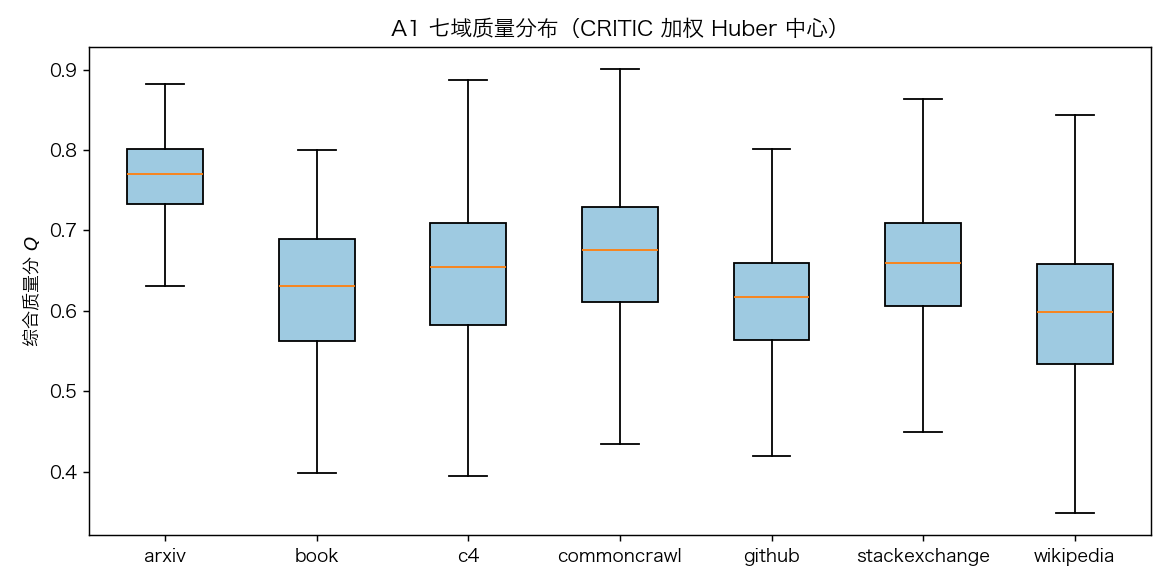
\includegraphics[width=.78\textwidth]{q1_F2_domain_quality_box.png}
\caption{A1 七个领域的 Huber 质量分呈现领域差异，同时抽样量较少的 book 分布更宽}
\label{fig:q1box}
\end{figure}

\subsubsection{质量冲突的定义、诊断与跨集复验}

评分完成后，按指标来源将 25 项指标划为 RPS（11 项）、DSIR（3 项）、轻量分类器（2 项）、FineWeb-Edu（1 项）、QuRating（4 项）和 ModernBERT（4 项）六个来源。对每篇文档，先用 A1 同域指标经验分布将标准化值转为中秩 $r_j(x)$，再计算来源内中位数 $m_s(x)$。在 A1 同域同来源的 $m_s$ 经验分布上再次取中秩，得到来源可比位置 $u_s(x)$。来源间分歧度定义为六个来源位置的极差：
\begin{equation}
r_j(x)=F_{dj}^{A1,\mathrm{mid}}\!\left(z_j(x)\right),\qquad
m_s(x)=\operatorname{median}_{j\in I_s}r_j(x),\qquad
u_s(x)=F_{ds}^{A1,\mathrm{mid}}\!\left(m_s(x)\right),\qquad
B(x)=\max_s u_s(x)-\min_s u_s(x).
\label{eq:q1_conflict}
\end{equation}
A1 每个领域 $B(x)$ 的第 95 百分位作为高分歧候选的筛查阈值；高端与低端立场分别指 $u_s\geq0.8$ 与 $u_s\leq0.2$。只有分歧超过阈值且高低两侧各至少有两个来源支持时，才称为“多来源对立候选”。A2/A3 冻结复用 A1 的单指标参照、来源参照和阈值。该 P95 是预先确定的筛查预算，A1 约 5\% 的候选比例不是实际冲突率。来源内部跨度、两端意见并存和单指标留一偏离另行诊断，避免来源中心掩盖内部异质性。

\begin{table}[H]
\centering\small
\caption{A1 冻结规则下三组数据的评分后分歧候选比例}
\label{tab:q1_conflict_rates}
\begin{tabular}{lrrr}
\toprule
数据集 & 高分歧候选 & 多来源对立候选 & 单指标独有候选\\
\midrule
A1 抽样集 & 5.00\% & 1.36\% & 5.62\%\\
A2 arxiv 全量 & 4.73\% & 1.58\% & 4.05\%\\
A3 github 全量 & 4.99\% & 1.77\% & 4.22\%\\
\bottomrule
\end{tabular}
\end{table}

A1 的来源内部诊断显示，六来源 Kendall $W$ 分别为 RPS 0.140、DSIR 0.967、轻量分类器 0.691、FineWeb-Edu（单指标，不适用）、QuRating 0.675、ModernBERT 0.579。文档内指标排名的 $P_{90}-P_{10}$ 中位数在 RPS 为 0.625，而 DSIR 为 0.037、QuRating 为 0.277、ModernBERT 为 0.315；另有 69.45\% 的文档在 RPS 指标中同时出现低于 20\% 与高于 80\% 的相对排名。这说明 RPS 来源内部异质性明显，来源中心本身不足以完整描述其信号。A1 的高分歧候选中，加权方向份额最大的来源对为“RPS 高、FineWeb-Edu 低”（8.03\%）；这是诊断方向分布，不足以确认冲突原因或任一来源更准确。

相同冻结规则在 A2、A3 上得到相近的高分歧候选比例；多来源对立候选分别占 1.58\% 和 1.77\%，单指标独有候选为 4.05\% 和 4.22\%。A2 中最高加权来源对为“ModernBERT 高、FineWeb-Edu 低”（9.89\%），A3 中为“RPS 高、FineWeb-Edu 低”（13.03\%）。以上均是候选筛查结果，且没有独立人工质量标签，不能据此称为实际冲突率、测量错误率或已确认成因。历史四来源口径的候选率为 19.08\%/24.52\%/23.28\%，其分组和阈值与现行六来源规则不同，只作为诊断对照；在 A1 前 5\% 配平预算后，旧新候选的 Jaccard 为 0.324/0.283/0.259，表示两种诊断筛选对象并不相同。

\begin{figure}[H]
\centering
\begin{minipage}{.48\textwidth}\centering
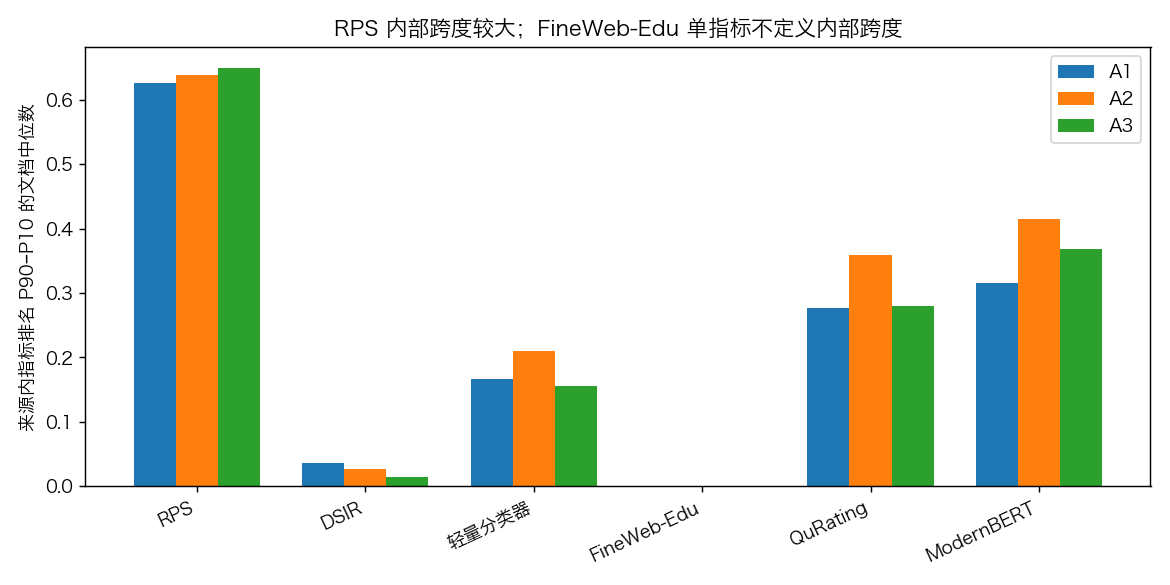
\includegraphics[width=\linewidth]{q1_F3_source_internal.png}
\caption{RPS 来源的域内指标差异大于其他多指标来源}
\label{fig:q1internal}
\end{minipage}\hfill
\begin{minipage}{.48\textwidth}\centering
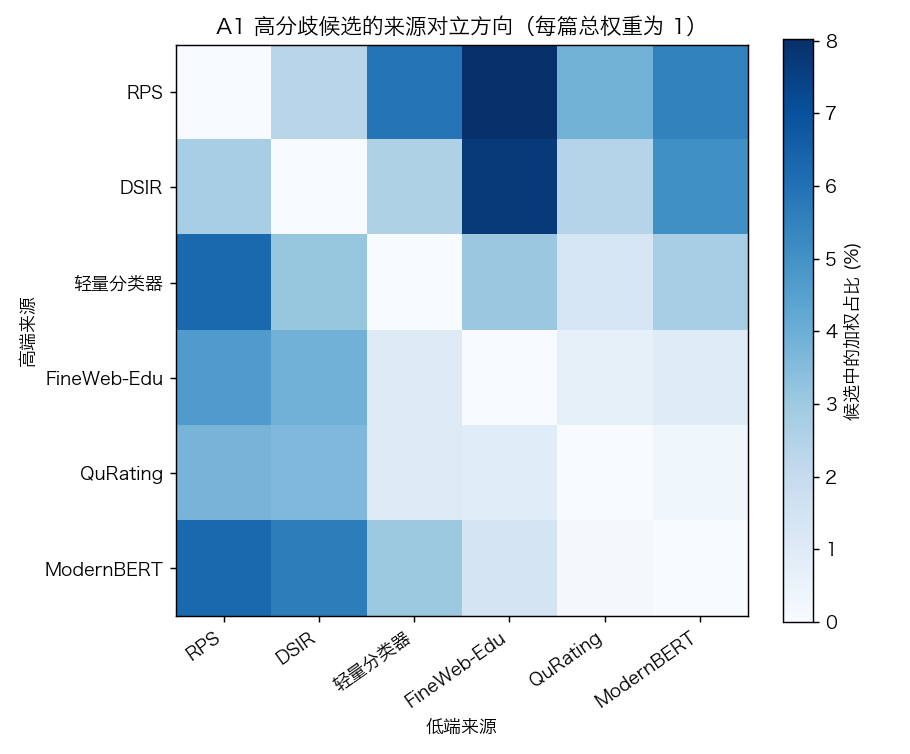
\includegraphics[width=\linewidth]{q1_F3_source_opposition.png}
\caption{六来源分析将高低立场组合拆分呈现}
\label{fig:q1opposition}
\end{minipage}
\end{figure}

\begin{figure}[H]
\centering
\begin{minipage}{.48\textwidth}\centering
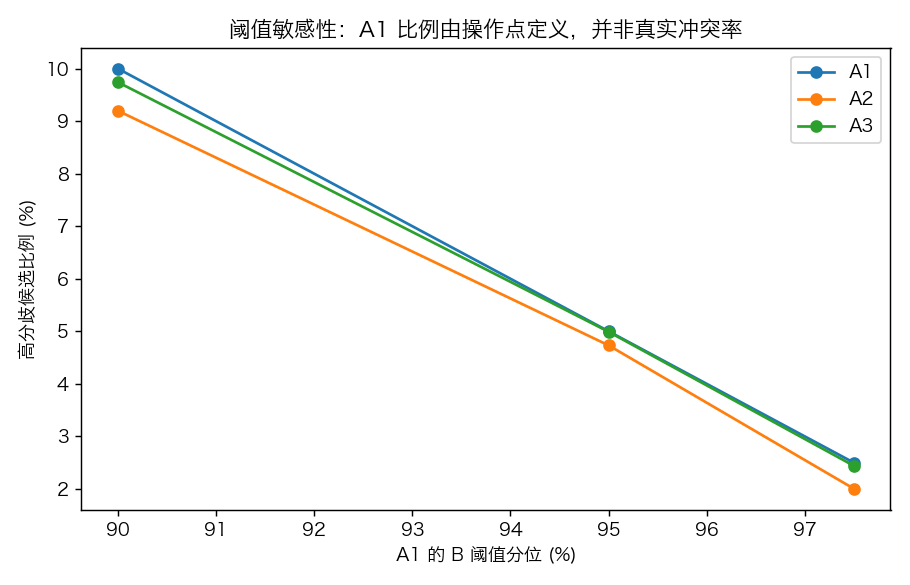
\includegraphics[width=\linewidth]{q1_F3_threshold_sensitivity.png}
\caption{A1 冻结分歧阈值改变候选筛查比例}
\label{fig:q1threshold}
\end{minipage}\hfill
\begin{minipage}{.48\textwidth}\centering
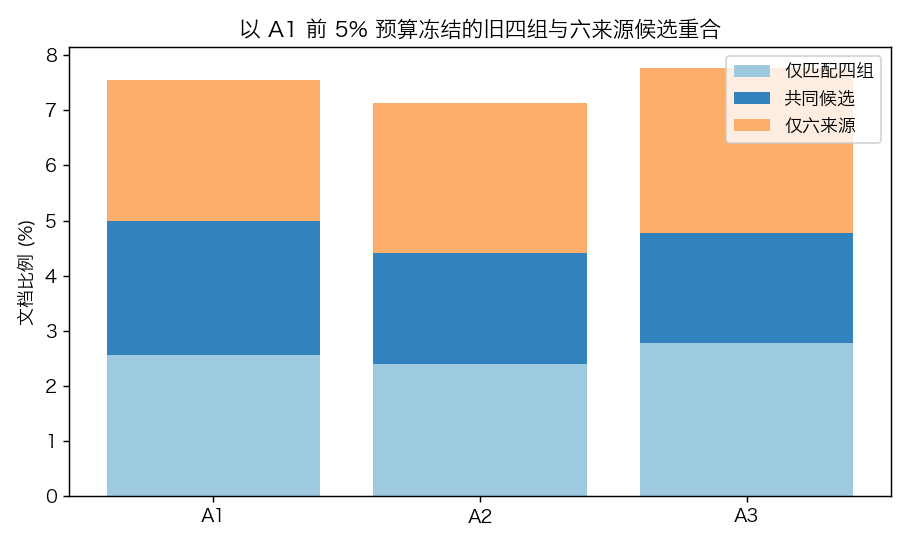
\includegraphics[width=\linewidth]{q1_F3_matched_overlap.png}
\caption{统一 A1 筛查预算后，旧四来源和六来源仍筛出不同文档}
\label{fig:q1matched}
\end{minipage}
\end{figure}

\paragraph{来源一致性加权对照实验}
为检验 §2.3 Kendall $W$ 所揭示的来源内部一致性差异是否影响质量排序，将原 CRITIC 权重 $w_j$ 乘以对应来源的 Kendall $W$ 后重新归一化：
\begin{equation}
\tilde w_j = w_j \cdot W_{s(j)}\bigg/\sum_{\ell=1}^{25}w_\ell\cdot W_{s(\ell)},
\label{eq:q1_wv2}
\end{equation}
再代入式~\eqref{eq:q1_huber} 的同一 Huber 二分法（$\delta=0.403491$ 不变，A2/A3 参数冻结），得到对照质量分 $Q_{\mathrm{v2}}$。权重变化方向与来源内部一致性一致：RPS（$W=0.140$）各指标均值权重由 0.0403 降至 0.0124；DSIR（$W=0.967$）由 0.0270 升至 0.0574；FineWeb-Edu（设 $W=1.0$）由 0.0359 升至 0.0790。

$Q_{\mathrm{v2}}$ 与主 $Q$ 的全局 Spearman 相关在 A1/A2/A3 分别为 \textbf{0.9547}、\textbf{0.9207}、\textbf{0.9395}，质量排序高度一致。A1 各域 $Q_{\mathrm{v2}}$ 中位数（降序）：arxiv 0.8009、commoncrawl 0.6428、stackexchange 0.6421、c4 0.6216、book 0.6012、github 0.5907、wikipedia 0.5408；域级排序与主 $Q$ 完全相同。对原四组冲突文档（$c_1\geq0.71$，9{,}776 条）与非冲突文档分别统计 $Q_{\mathrm{v2}}-Q$ 分布，两组存在可见差异，但差异量级较小，不足以说明来源一致性加权对冲突文档有专向修正效果。Spearman 仅衡量排序相似度，$Q_{\mathrm{v2}}$ 是实验性对照分，不替换主质量口径 $Q$，也不更新任何 P1 接口。

\begin{figure}[H]
\centering
\begin{minipage}{.48\textwidth}\centering
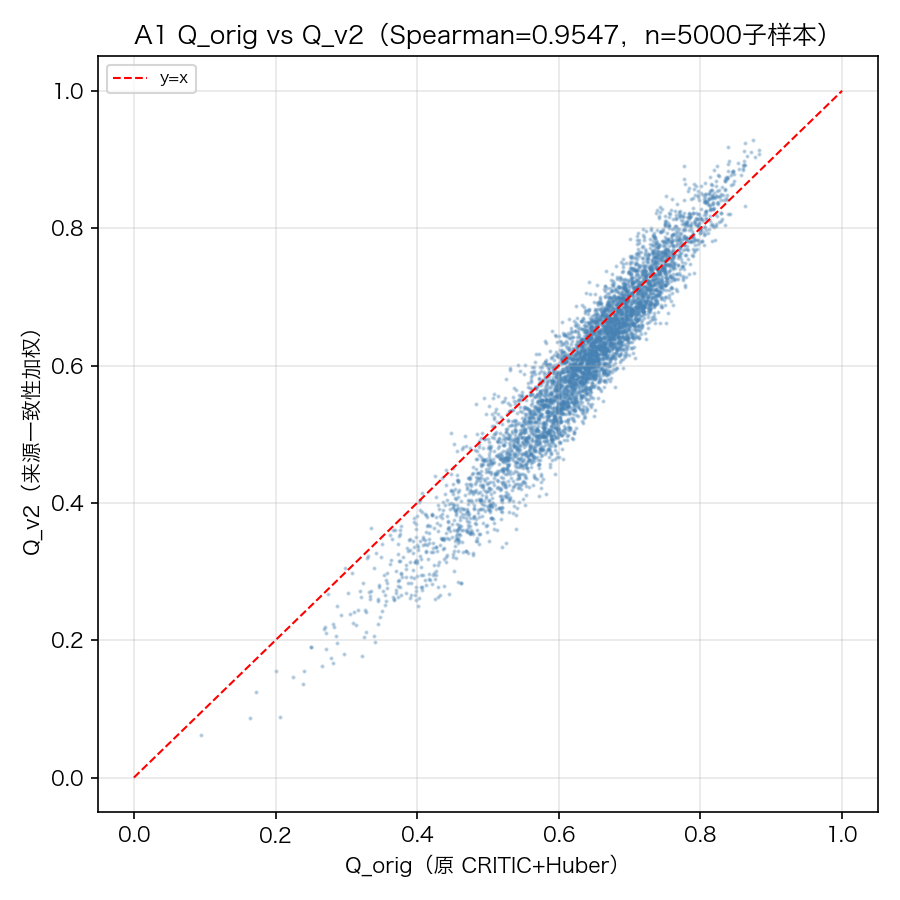
\includegraphics[width=\linewidth]{q1_F3_Q_v2_scatter_A1.png}
\caption{A1 上 $Q_{\mathrm{v2}}$ 与主 $Q$ 的散点分布（Spearman = 0.9547）}
\label{fig:q1v2scatter}
\end{minipage}\hfill
\begin{minipage}{.48\textwidth}\centering
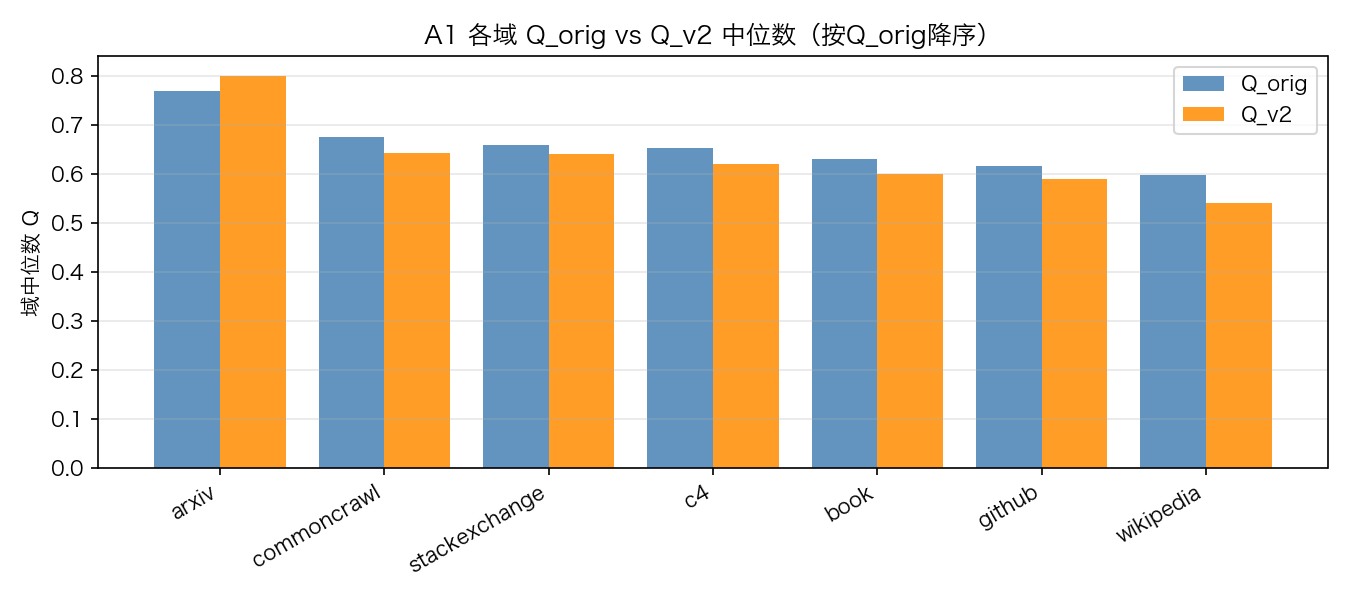
\includegraphics[width=\linewidth]{q1_F3_Q_v2_domain_median.png}
\caption{A1 各域 $Q_{\mathrm{v2}}$ 与主 $Q$ 中位数对比，域级排序不变}
\label{fig:q1v2domain}
\end{minipage}
\end{figure}

\subsubsection{17 域配比、交叉熵损失及质量关系建模}

\paragraph{从七个质量领域桥接到十七个配比领域}
A16 将 17 个配比领域对应为 3 个 direct、3 个 near\_direct 和 11 个 inferred 域。对 6 个 direct/near\_direct 域，直接采用映射到的 A1 域主质量分中位数及其 bootstrap 区间；对 11 个 inferred 域，以 A1 的 21{,}590 篇可用原文和同一主 $Q$ 为训练标签，使用 11 个可复算的规则特征进行按领域分层五折选型，再将选出的 GBDT 应用于 A18 的 31{,}340 篇有效文档，按配比域取预测中位数及文档 bootstrap 区间。五折均值 $R^2=0.4106$（Ridge 对照为 0.3415）；在 6 个映射域上的 Pearson 相关为 0.6549、Spearman 相关为 0.7714、MAE 为 0.0365（$n=6$）。17 域中 arxiv 最高（0.7707），dm\_mathematics 最低（0.5091）。映射区间以 A16 对应关系成立为条件，inferred 区间不含桥接模型选择及跨域偏差；ubuntu\_irc（16 篇）和 philpapers（63 篇）需谨慎使用。

\begin{figure}[H]
\centering
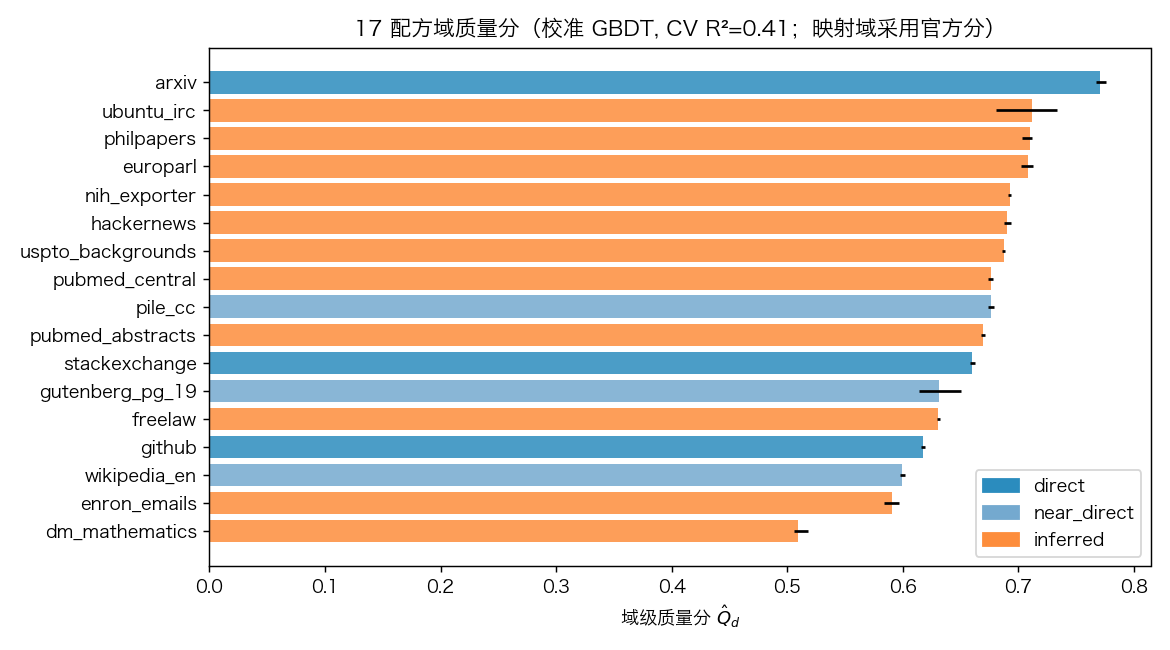
\includegraphics[width=.86\textwidth]{q1_F4_bridge_17domains.png}
\caption{17 域质量分依据映射等级取直接评分或桥接预测，误差条为同源 bootstrap 区间}
\label{fig:q1bridge}
\end{figure}

\paragraph{十七域配比与验证交叉熵的定量关系}
A4、A5 分别提供 512 组训练配比和 13 个验证域的交叉熵损失，按 \texttt{index} 连接。对配比向量 $\bp=(p_1,\ldots,p_{17})$ 中非正份额以 $10^{-4}$ 替代并重新闭合，再作中心对数比变换：
\begin{equation}
\operatorname{clr}(\bp)_i=\log p_i-\frac{1}{17}\sum_{k=1}^{17}\log p_k,\qquad
\log L_v=b_v+\sum_{i=1}^{17}\beta_{vi}\operatorname{clr}(\bp)_i+\varepsilon_v,\quad v=1,\ldots,13.
\label{eq:clr}
\end{equation}
主解释模型为逐验证域 Huber 回归，原始份额 OLS 和 GBDT 用作对照。由线性模型在均匀配比处求导，得到 $17\times13$ 的局部迁移矩阵：
\begin{equation}
T_{iv}=17\left(\beta_{vi}-\bar\beta_v\right),\qquad
\bar\beta_v=\frac{1}{17}\sum_{i=1}^{17}\beta_{vi}.
\label{eq:q1_transfer}
\end{equation}
在 A6/A7 的 1M 留出集上，三个模型的平均逐域 $R^2$ 分别为 clr+Huber 0.772、裸配比 OLS 0.654、GBDT 0.897。对 13 域等权综合目标，clr+Huber 的 $R^2$ 为 0.260，裸 OLS 为 0.418；因此 clr+Huber 的优势体现在逐域拟合与系数解释，不是每个汇总目标上都更优。GBDT 作为非线性对照并用于候选配比预测。

\begin{figure}[H]
\centering
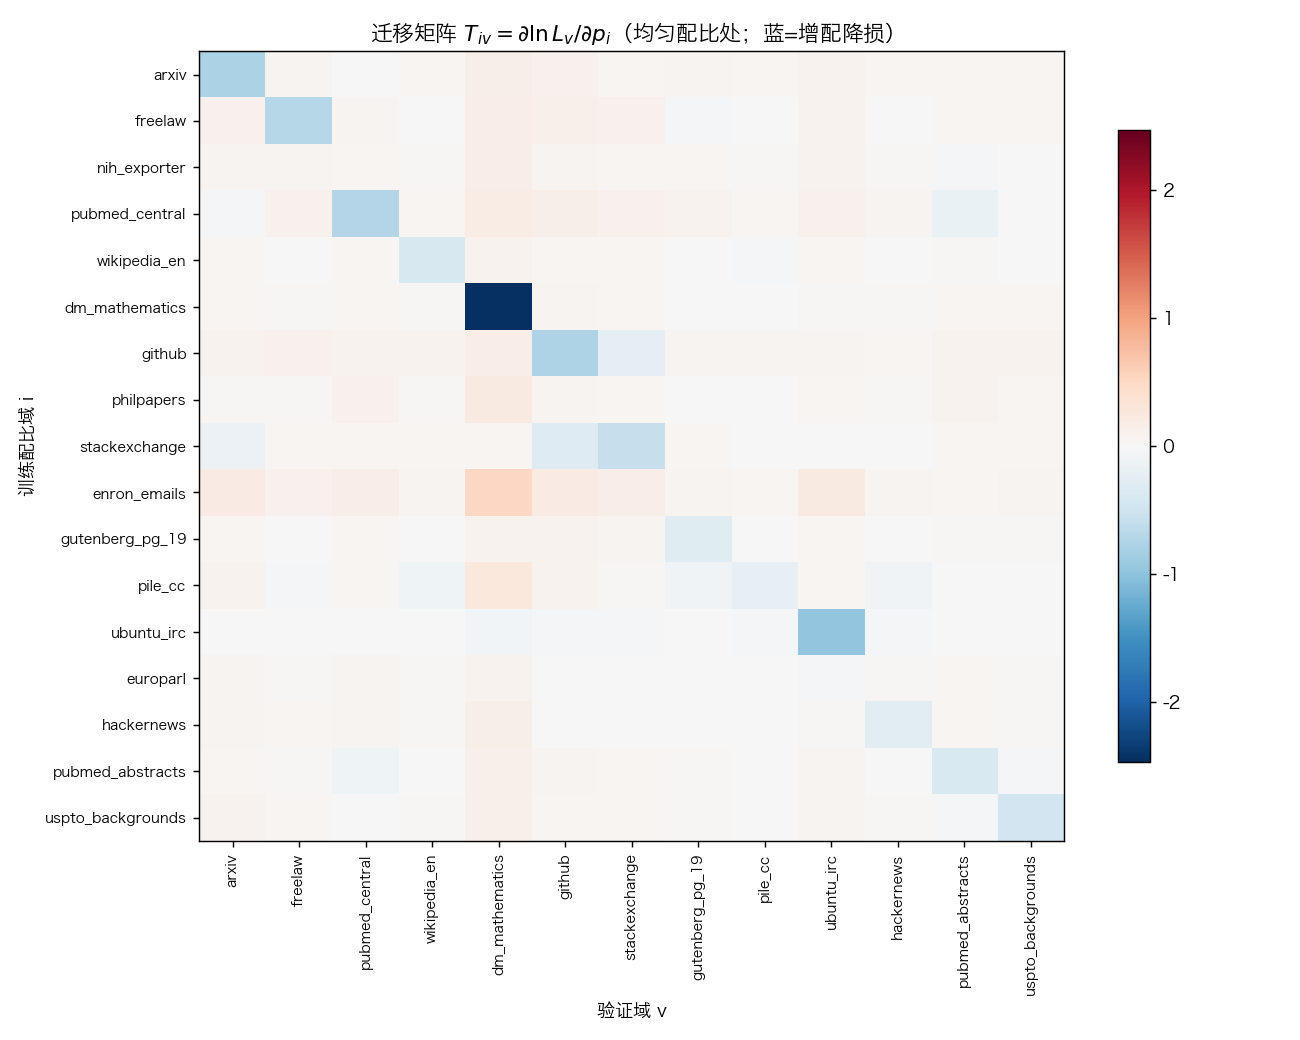
\includegraphics[width=.84\textwidth]{q1_F5_transfer_matrix.png}
\caption{均匀配比附近的迁移矩阵显示增配不同领域对各验证域损失的局部影响}
\label{fig:q1tm}
\end{figure}

\paragraph{配比与质量的关系及候选配比}
17 域质量分沿用前述直接映射或桥接的 $Q_i$。配比下的加权平均质量及其与验证损失的附加关系分别表示为
\begin{equation}
\bar Q(\bp)=\sum_{i=1}^{17}p_iQ_i,\qquad
\log L_v=b_v+\sum_{i=1}^{17}\beta_{vi}\operatorname{clr}(\bp)_i
+\lambda_v\sum_{i=1}^{17}p_i(1-Q_i)+\varepsilon_v.
\label{eq:q1_pq}
\end{equation}
质量交互项以 400 次案例 bootstrap 评估，13 个验证域中仅 6 个区间不含零，且系数有正有负；它是关联分析，不能解释为质量的因果效应。17 域 $Q_i$ 与训练边际价值的 Spearman 相关为 $-0.211$，样本量有限，说明质量排序不能替代配比实验。

以 A4 平均配比为中心，从四档浓度 Dirichlet 分布生成 99{,}996 个候选，由 GBDT 分别按 13 域等权损失和 pile\_cc 单域损失评分，取各自前 100 个候选的平均配比。等权候选的头部领域为 pile\_cc 15.5\%、stackexchange 10.0\%、wikipedia\_en 9.5\%、pubmed\_central 9.1\%、arxiv 8.9\%。等权候选、pile\_cc 候选与均匀配比的当前加权质量分别为 0.6609、0.6603 和 0.6606。相较均匀配比，GBDT 预测降损为 9.915\%；固定候选后，线性模型 bootstrap 的收益中位数为 11.90\%，95\% 区间为 [9.72\%,14.12\%]。两项分别来自不同模型，后者不是 GBDT 点估计的置信区间。

pile\_cc 单域候选经前百平均后，其自身目标 Loss 为 5.608，高于等权候选的 5.530；因此两组份额均作为搜索候选报告，不能把平均后的 pile\_cc 份额称为复评最优解。以上降损也只是代理模型预测，尚未经重新训练实测。

\begin{figure}[H]
\centering
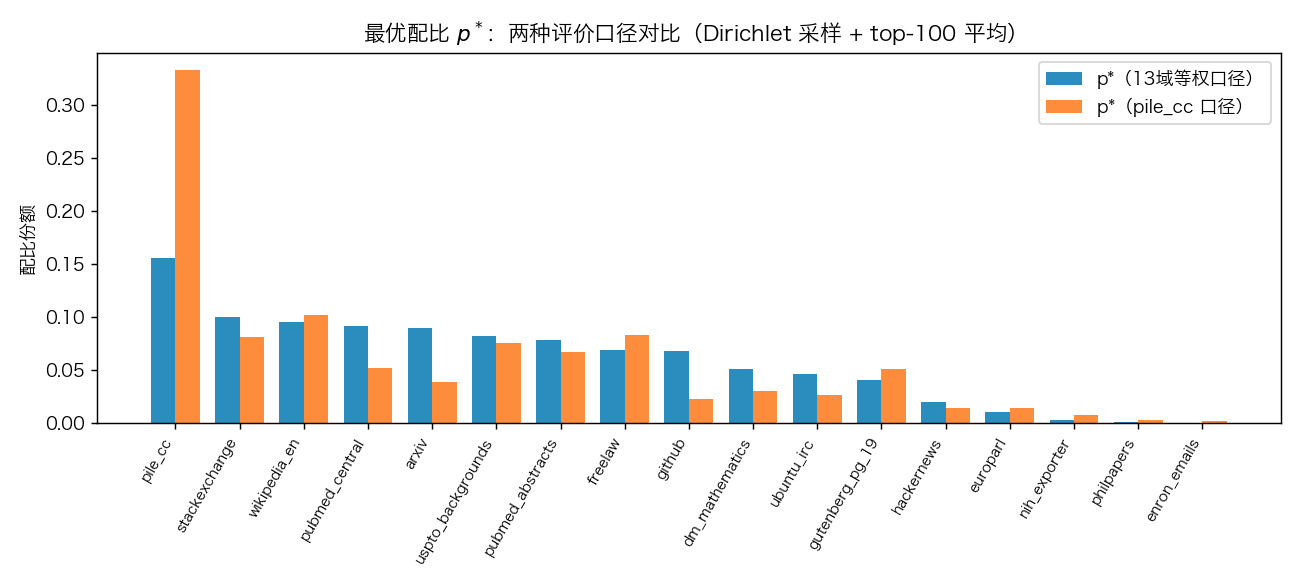
\includegraphics[width=.92\textwidth]{q1_F7_p_star.png}
\caption{两种损失目标对应不同的候选配比}
\label{fig:q1pstar}
\end{figure}

\begin{figure}[H]
\centering
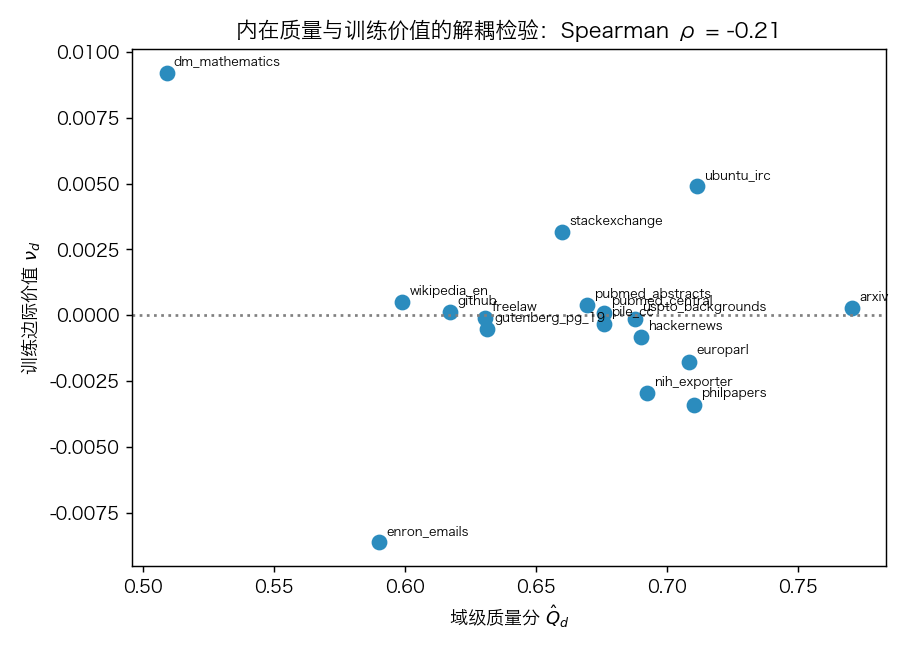
\includegraphics[width=.82\textwidth]{q1_F7_quality_vs_value.png}
\caption{17 域质量与训练边际价值的秩相关较弱}
\label{fig:q1qv}
\end{figure}

\paragraph{A6--A11 检验与 A12--A15 外推稳健性}
\label{sec:q1-scale}
用 A4/A5 拟合的 1M 线性模型冻结预测 A6/A7 的 1M 留出集、A8/A9 的 60M 集和 A10/A11 的 1B 集，目标损失排序 Spearman 分别为 0.523、0.467、0.677。60M 和 1B 的绝对损失预测失效（平均逐域 $R^2$ 分别为 $-7.69$ 和 $-604.66$），所以排序保持不代表绝对量可迁移；1B 检验集只有 64 组。

A12--A15 的 10B、70B 表均为估算/外推值，不是实际训练观测。在这些表上直接套用 1M 系数，MAE 分别为 3.53 和 3.91，Spearman 为 $-0.532$ 和 $-0.588$；再按观测尺度系数漂移作修正后，MAE 降为 0.104 和 0.108，但 Spearman 仍为 $-0.089$ 和 $-0.040$。这仅表明估算表上的绝对误差对漂移修正较敏感，不构成对真实大规模训练的外部验证，也不支持稳健排序外推。

\begin{figure}[H]
\centering
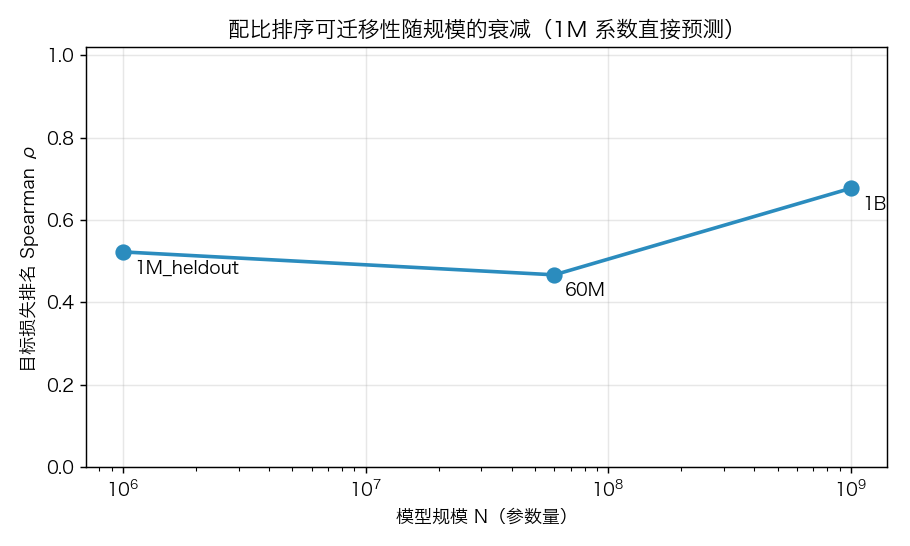
\includegraphics[width=.68\textwidth]{q1_F6_rank_decay.png}
\caption{冻结 1M 模型在观测尺度上只保留有限的配比排序能力}
\label{fig:q1rank}
\end{figure}

\subsection{问题二的模型建立与求解}

\subsubsection{模型建立}

\textbf{建模思路。}经典标度律只有 $N$ 与 $D$ 两个变量。本文采用\emph{基线 + 质量修正}的结构：先在附件内锚定经典项，再让数据决定质量以何种形式进入。候选形式分两族。第一族是\textbf{加性惩罚族}，质量不足直接抬高损失；第二族是文献常用的\textbf{有效数据乘子族}，低质量数据折算为更少的有效 token\cite{muennighoff}。两族在经济含义上不同：前者意味着低质量带来规模无法弥补的损失，后者意味着多读数据总能弥补质量不足。

\textbf{数据审计与逆向。}B1 可被三参数形式拟合到 $\mathrm{RMSE}=1.5\times10^{-4}$，是公式生成的无噪声锚点。在 B6/B7 的 $N\times D\times Q$ 网格上，残差去除基线后与 $(1-Q)$ 呈线性关系，且斜率随 $N^{-0.34}$ 衰减（图~\ref{fig:q2rev}）。据此逆向得到的生成式为“基线 $+\,(1-Q)(0.19+175N^{-0.34})$”。B8 与 B6/B7 在相同 $(N,D,Q)$ 点上的相关系数为 $-0.03$，语义不同源，因此不参与联合拟合。

\begin{figure}[H]
\centering
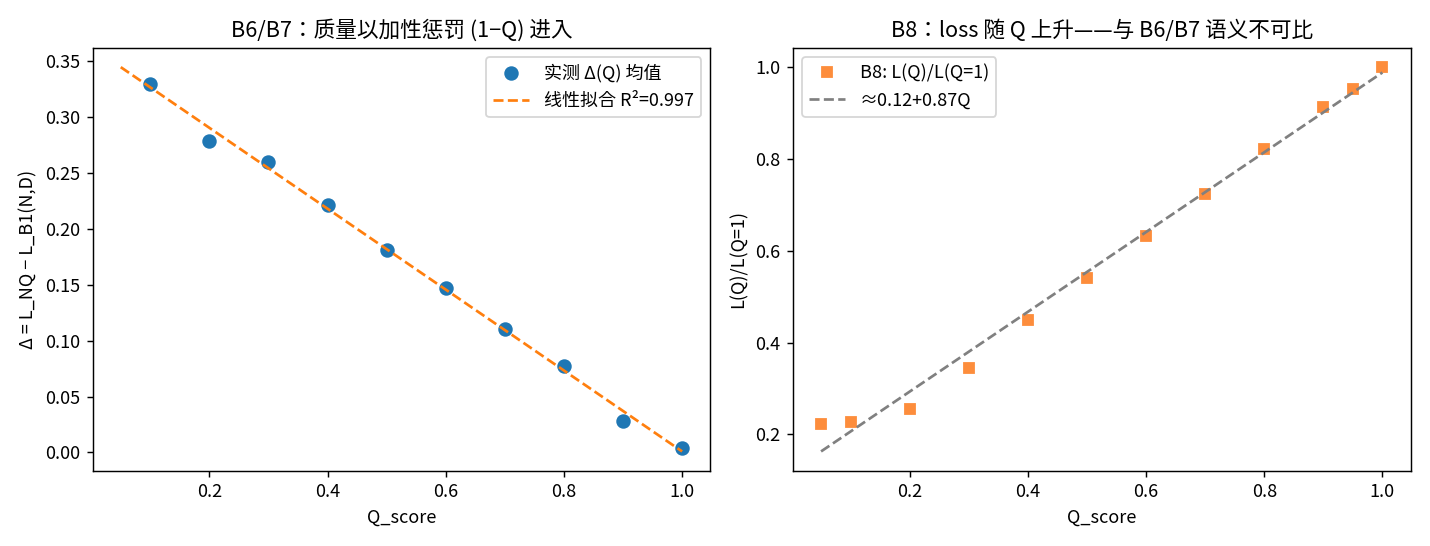
\includegraphics[width=.95\textwidth]{q12_F8_reverse_engineering.png}
\caption{附件 B 的逆向分析：B1 锚点（左）、B6/B7 残差对 $(1-Q)$ 的线性结构（中）、B8 与 B6/B7 的不一致（右）}
\label{fig:q2rev}
\end{figure}

\textbf{主模型。}交叉验证选型后（见 5.3.2 节），广义标度律为
\begin{equation}
\boxed{\;L(N,D,Q)=E+\widetilde A(Q)\,N^{-\alpha}+B\,D^{-\beta}+(1-Q)\,k_0,\qquad
\widetilde A(Q)=A+k_1(1-Q)\;}
\label{eq:main}
\end{equation}
$Q=1$ 时式~\eqref{eq:main} 严格退化为经典 Chinchilla 形式\cite{hoffmann}。$k_0$ 项是不随规模衰减的“质量地板”，$k_1$ 项是随 $N^{-\alpha}$ 衰减的“质量—规模交互”。

\textbf{配比的接入。}按赛题要求，问题二不重复读取附件 A，配比只通过问题一的接口进入：
\begin{equation}
Q_{\mathrm B}(\bp)=\frac{1}{Q_{\mathrm{ref}}}\sum_{i=1}^{17}p_i\,\hat Q_{d(i)},\qquad Q_{\mathrm{ref}}=\bar Q(\bp_{\mathrm{pile}})=0.5608,
\label{eq:qmix}
\end{equation}
即把配比映射为语料平均质量后代入 $Q$。配比的域结构效应（哪个域帮哪个验证域）由迁移矩阵 $T$ 单独描述。问题一已发现交互系数 $\lambda_v$ 的符号在域间不一致，因此不把质量与配比合并为单一乘子。

\subsubsection{求解方法}

\textbf{两步拟合。}第一步在 B1 上网格搜索 $(\alpha,\beta)$，再以最小二乘确定 $(E,A,B)$，得到 $L_0=1.6901+406.4N^{-0.340}+410.6D^{-0.280}$。第二步固定基线，在 B6/B7 的 450 个点上对五种候选质量项做五折交叉验证（表~\ref{tab:forms}）。参数区间用残差 bootstrap（$B=500$）估计。

\begin{table}[H]
\centering\small
\caption{质量项形式选择（五折 cv-RMSE；数据噪声水平 $\sigma\approx0.05$）}
\label{tab:forms}
\begin{tabular}{llc}
\toprule
候选形式 & 所属族 & cv-RMSE \\
\midrule
\textbf{加性 + 规模交互}\ $(1-Q)(k_0+k_1N^{-\alpha})$ & 加性惩罚 & $\mathbf{0.0512}$ \\
纯加性\ $k(1-Q)$ & 加性惩罚 & $0.0731$ \\
指数乘子\ $D_{\mathrm{eff}}=De^{-\gamma(1-Q)}$ & 有效数据乘子 & $0.0985$ \\
线性乘子\ $D_{\mathrm{eff}}=D\,(q_0+(1-q_0)Q)$ & 有效数据乘子 & $0.1030$ \\
幂律乘子\ $D_{\mathrm{eff}}=DQ^{\gamma}$ & 有效数据乘子 & $0.1050$ \\
\bottomrule
\end{tabular}
\end{table}

主模型的 cv-RMSE 达到数据噪声水平，而文献偏好的有效数据乘子族全部落败。模型形式由交叉验证裁决，而不是从文献先验借用。

\begin{table}[H]
\centering\small
\caption{广义标度律参数估计（括号内为残差 bootstrap 95\% CI）}
\label{tab:params}
\begin{tabular}{cccccccc}
\toprule
$E$ & $A$ & $\alpha$ & $B$ & $\beta$ & $k_0$ & $k_1$ & 残差 $\sigma$ \\
\midrule
$1.6901$ & $406.39$ & $0.34$ & $410.59$ & $0.28$ &
\makecell{$0.1922$\\ {\footnotesize$[0.175,0.211]$}} & \makecell{$175.29$\\ {\footnotesize$[156.6,193.0]$}} & $0.051$ \\
\bottomrule
\end{tabular}
\end{table}

\subsubsection{结果与分析}

\textbf{跨源检验。}在真实文献点上，主模型预测与观测的 Spearman 相关为：scaling\_baseline（57 点）$0.983$，published（44 点）$0.959$；平均偏差分别为 $0.22$ 与 $0.02$ nats。趋势一致，绝对偏移来自 tokenizer 与验证集差异，符合“跨源只比趋势”的原则。B2（半合成）Spearman 为 $0.788$、偏差为 $1.18$ nats，仅作定性佐证。

\textbf{解析命题。}以下四条命题均由式~\eqref{eq:main} 直接推出，并与数值优化互验：命题~\ref{prop:sub} 为逐点代入，命题~\ref{prop:opt} 与数值最优解的最大相对误差 $<10^{-5}$。

\begin{proposition}[弹性]\label{prop:el}
损失对三个因素的弹性为
$\displaystyle
\varepsilon_N=-\frac{\alpha\widetilde A(Q)N^{-\alpha}}{L},\quad
\varepsilon_D=-\frac{\beta BD^{-\beta}}{L},\quad
\varepsilon_Q=-\frac{Q(k_0+k_1N^{-\alpha})}{L}.$
在 $(N,D,Q)=(10^{10},10^{12},0.9)$ 处三者依次为 $-0.028$、$-0.024$、$-0.115$，即\emph{质量弹性约为规模弹性的 4 倍}。由于 $k_0$ 项不随 $N$ 衰减，规模越大，质量的相对优势越明显。
\end{proposition}

\begin{proposition}[质量—参数等效替代及其边界]\label{prop:sub}
固定 $D$，使 $L(N',D,Q)=L(N,D,Q+\delta)$ 成立的等效参数量为
\begin{equation}
N'=N\Bigl[1-\frac{\delta\,(k_0+k_1N^{-\alpha})}{\widetilde A(Q)N^{-\alpha}}\Bigr]^{-1/\alpha},
\end{equation}
当且仅当括号内为正时有限。质量从 $0.9$ 提高到 $1.0$，在 $N=10^9$ 处等效于参数扩大 $1.33$ 倍，在 $N=10^{10}$ 处等效于扩大 $1.64$ 倍（bootstrap 区间 $[1.52,1.77]$）。同一份质量改进，模型越大价值越高；超过临界规模后，任何有限的扩参都无法替代这次质量提升。这就是“质量与规模可相互替代”的条件。
\end{proposition}

\begin{proposition}[质量地板]\label{prop:fl}
$\lim_{N,D\to\infty}L=E+(1-Q)k_0$。低质量会带来规模无法弥补的损失下界：$Q=0.5$ 的地板比 $Q=1$ 高 $0.096$ nats。这为问题三的“付费提质”提供了理论依据。
\end{proposition}

\begin{proposition}[算力最优配置随质量移动]\label{prop:opt}
在约束 $6ND=C$ 下，
\begin{equation}
N^{*}(C,Q)=\Bigl[\frac{\alpha\widetilde A(Q)}{\beta B}\Bigr]^{\frac{1}{\alpha+\beta}}
\Bigl(\frac{C}{6}\Bigr)^{\frac{\beta}{\alpha+\beta}},\qquad \frac{\beta}{\alpha+\beta}=0.452,
\qquad \frac{\partial N^{*}}{\partial Q}<0 .
\label{eq:nstar}
\end{equation}
质量越高，最优配置越偏向“小模型、多数据”：$C=10^{22}$ 时，最优 token/参数比由 $Q=0.3$ 时的 27 升至 $Q=1$ 时的 63。其机制是低质量数据抬高了 $\widetilde A(Q)$，相当于提高了参数的边际收益。这一命题是问题三结构性转移的机制来源。
\end{proposition}

\begin{figure}[H]
\centering
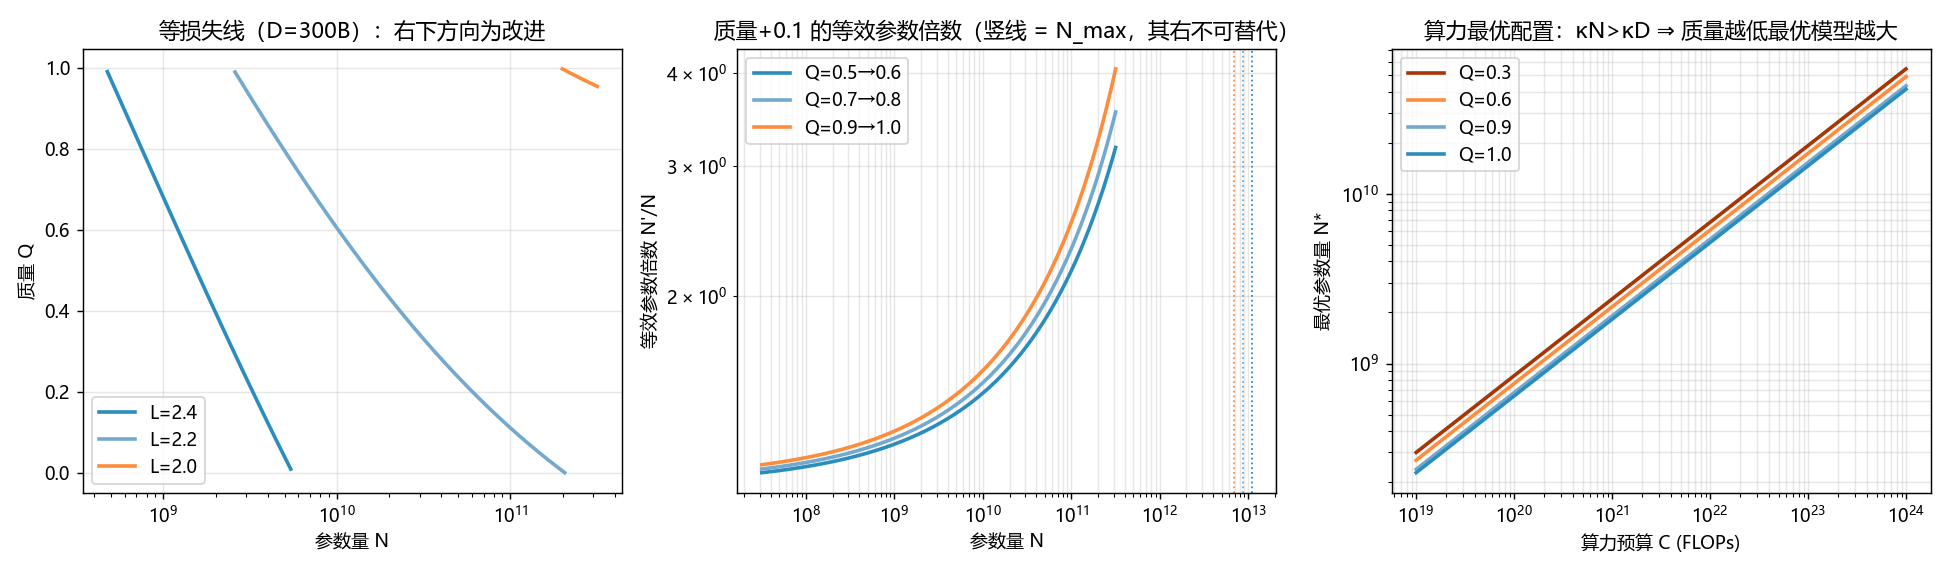
\includegraphics[width=\textwidth]{q12_F21_theory.png}
\caption{解析理论三联图：等损失线（左）、等效参数倍数（中）、$N^*(C,Q)$（右）}
\label{fig:theory}
\end{figure}

\textbf{领域间的替代与互补。}广义律中的配比通道由两部分组成。第一部分是 $Q_{\mathrm B}(\bp)$：把质量高的域（arxiv、stackexchange）换入，会通过 $(1-Q)$ 两项同时降损。第二部分是迁移矩阵 $T$（表~\ref{tab:q2tm}）：13 个自域效应全部为负，说明各域“自己补自己”最有效；非对角的负值对应\textbf{互补}，最典型的是 github 与 stackexchange 双向互补（$-0.21/-0.32$），pubmed\_central 与 pubmed\_abstracts 双向互补（$-0.16/-0.11$），pile\_cc 增配也会降低 wikipedia 的损失（$-0.11$）；正值对应\textbf{替代}（挤占），最典型的是 dm\_mathematics 列除 ubuntu\_irc 外全为正（$0.04$–$0.50$），即几乎任何其他域的增配都会挤占数学能力，enron\_emails 增配则使全部 13 个验证域的损失上升。第二部分主导配比效应，这一点在问题三的联立优化中得到印证（5.4.3 节）：联合降损几乎全部来自配比结构，而不是 $Q_{\mathrm B}(\bp)$ 通道。

\begin{table}[H]
\centering\small
\caption{迁移矩阵 $T_{iv}$ 中的代表性互补与替代关系（节选）}
\label{tab:q2tm}
\begin{tabular}{llcl}
\toprule
增配域 $i$ & 验证域 $v$ & $T_{iv}$ & 关系 \\
\midrule
stackexchange & github & $-0.32$ & 互补（问答 $\to$ 代码） \\
github & stackexchange & $-0.21$ & 互补（代码 $\to$ 问答） \\
pubmed\_central & pubmed\_abstracts & $-0.16$ & 互补（全文 $\to$ 摘要） \\
stackexchange & arxiv & $-0.15$ & 互补 \\
pile\_cc & wikipedia\_en & $-0.11$ & 互补（网页 $\to$ 百科） \\
enron\_emails & dm\_mathematics & $+0.50$ & 替代（挤占） \\
pile\_cc & dm\_mathematics & $+0.26$ & 替代（挤占） \\
\bottomrule
\end{tabular}
\end{table}

\subsection{问题三的模型建立与求解}

\subsubsection{模型建立}

\textbf{优化问题。}以问题二的广义标度律式~\eqref{eq:main} 为目标，建立
\begin{equation}
\begin{aligned}
\min_{N,D,Q}\ & L(N,D,Q)\\
\text{s.t.}\ & 6ND+D\,[g(Q)-g(Q_0)]_{+}+\eta\,N D L_{\mathrm{ctx}}\le C,\qquad Q_0\le Q\le1,
\end{aligned}
\label{eq:q3}
\end{equation}
其中 $\eta=2\times10^{-4}$。三种单位 token 提质成本函数为：指数型 $g_1=10^7e^{6Q}$，幂函数型 $g_2=5\times10^9Q^4$，对数型 $g_3=2\times10^9\ln(1+10Q)$。基线质量 $Q_0$ 取两个口径：主口径为 $\bp^*$ 加权质量按式~\eqref{eq:qmix} 换算，$Q_0=0.9878$；副口径取网页语料 c4，$Q_0=0.8892$。

\textbf{降维。}三项成本都与 $D$ 成正比，而 $L$ 对 $D$ 严格递减，所以最优时预算约束必取等。记 $\kappa=6+\eta L_{\mathrm{ctx}}$、$\Delta g(Q)=[g(Q)-g(Q_0)]_+$，则
\begin{equation}
D(N,Q)=\frac{C}{\kappa N+\Delta g(Q)},
\label{eq:dsolve}
\end{equation}
代回后，式~\eqref{eq:q3} 化为 $(\log N,Q)$ 上的二维\emph{无约束}问题，不需要罚函数。

\textbf{上下文长度的解析临界值。}注意力项与训练项之比为 $\eta L_{\mathrm{ctx}}/6$，二者相等时
\begin{equation}
L_{\mathrm{ctx}}^{\mathrm{crit}}=6/\eta=30000 .
\end{equation}
在不提质区域，把式~\eqref{eq:nstar} 中的 $6$ 换成 $\kappa$ 即得闭式解 $N^*\propto(C/\kappa)^{\beta/(\alpha+\beta)}$，因此
\begin{equation}
N^*(L_{\mathrm{ctx}})\,/\,N^*(2048)=\bigl[(6+2048\eta)/\kappa\bigr]^{0.452}.
\label{eq:ctxratio}
\end{equation}

\textbf{结构性转移的定义。}
\begin{definition}[结构性转移]\label{def:st}
记 $x^*(C)=(N^*,D^*,Q^*)$ 为预算 $C$ 下的最优解，其 KKT 活跃约束集 $\mathcal A(C)$ 有三种状态：$\{Q\ge Q_0\}$ 活跃（不提质）、内点（部分提质）、$\{Q\le1\}$ 活跃（提满）。若 $\mathcal A(C)$ 在 $C_{\mathrm{crit}}$ 两侧不同，则称预算在 $C_{\mathrm{crit}}$ 处发生\textbf{结构性转移}。
\end{definition}

在 $Q=Q_0$ 处，“提质的边际收益”与“提质挤占数据的边际损失”之比为
\begin{equation}
\Phi(C)=\frac{(k_0+k_1N^{-\alpha})\,(\kappa N+\Delta g)}{\beta B\,D^{-\beta}\,g'(Q)}\Bigg|_{x^*(C)} .
\label{eq:phi}
\end{equation}
$\Phi<1$ 时，不提质就是 KKT 点；$\Phi(C)=1$ 的解就是 $C_{\mathrm{crit}}$，用二分法求得（口径 A）。另设两个辅助口径：口径 B 取提质成本占比 $s_Q$ 的峰值点；口径 C 取 $D^*/N^*$ 的对数斜率偏离常数 $(\alpha-\beta)/(\alpha+\beta)$ 最大的点。

\subsubsection{求解方法}

内层对 $\log N$ 做黄金分割搜索（剖面损失关于 $N$ 单峰），外层对 $Q$ 做三级网格加密，最终步长小于 $10^{-5}$，并对端点 $Q_0$ 与 $1$ 做保护。求解器全向量化（附录 A.2）。求解范围为：3 种 $g$ × 7 档预算（$10^{19}$–$10^{25}$）× 5 档 $L_{\mathrm{ctx}}$（取 C7 中的可行值 2k/4k/8k/32k/128k）× 2 种 $Q_0$，共 210 组。

求解器做两项互验。在 $\Delta g=0$ 的 15 组中，数值解与闭式 $N^*$ 的相对误差不超过 $1.83\times10^{-7}$；与粗网格穷举对比的 18 组中，Loss 差不超过 $1.6\times10^{-5}$，且区制判定一致。稳健性部分对问题二的 500 组 bootstrap 参数逐组重解 $C_{\mathrm{crit}}$，并对 $\eta$ 做 $\pm50\%$ 扰动。

\subsubsection{结果与分析}

\textbf{关键预算下的最优配置。}表~\ref{tab:q3key} 给出主口径、指数型、$L_{\mathrm{ctx}}=2048$ 的结果。$D^*/N^*$ 由 31 升至 97，符合 $\alpha>\beta$ 时“数据增长快于参数”的规律。提质只占很小的成本份额（$<1\%$），却带来最优解的区制变化。

\begin{table}[H]
\centering\small
\caption{关键预算下的最优配置（主口径 $Q_0=0.9878$，指数型，$L_{\mathrm{ctx}}=2048$）}
\label{tab:q3key}
\begin{tabular}{cccccccl}
\toprule
$C$ & $N^*$ & $D^*$ & $Q^*$ & $L^*$ & $D^*/N^*$ & $s_Q$ & 区制 \\
\midrule
$10^{19}$ & $2.23\times10^{8}$ & $6.99\times10^{9}$ & $0.9878$ & $3.004$ & $31.3$ & $0$ & 不提质（$Q_0$ 角点） \\
$10^{22}$ & $5.06\times10^{9}$ & $3.06\times10^{11}$ & $1$ & $2.144$ & $60.4$ & $0.87\%$ & 提满（$Q=1$ 角点） \\
$10^{24}$ & $4.01\times10^{10}$ & $3.88\times10^{12}$ & $1$ & $1.914$ & $96.7$ & $0.11\%$ & 提满 \\
\bottomrule
\end{tabular}
\end{table}

幂函数型结果与表~\ref{tab:q3key} 几乎相同；对数型在 $10^{19}$ 就已提满（$L^*=3.002$）。副口径起点质量更低，提质更划算：$C=10^{22}$ 时，指数型与幂函数型的 $s_Q$ 约为 $5.4\%$，对数型为 $0.65\%$。

\begin{figure}[H]
\centering
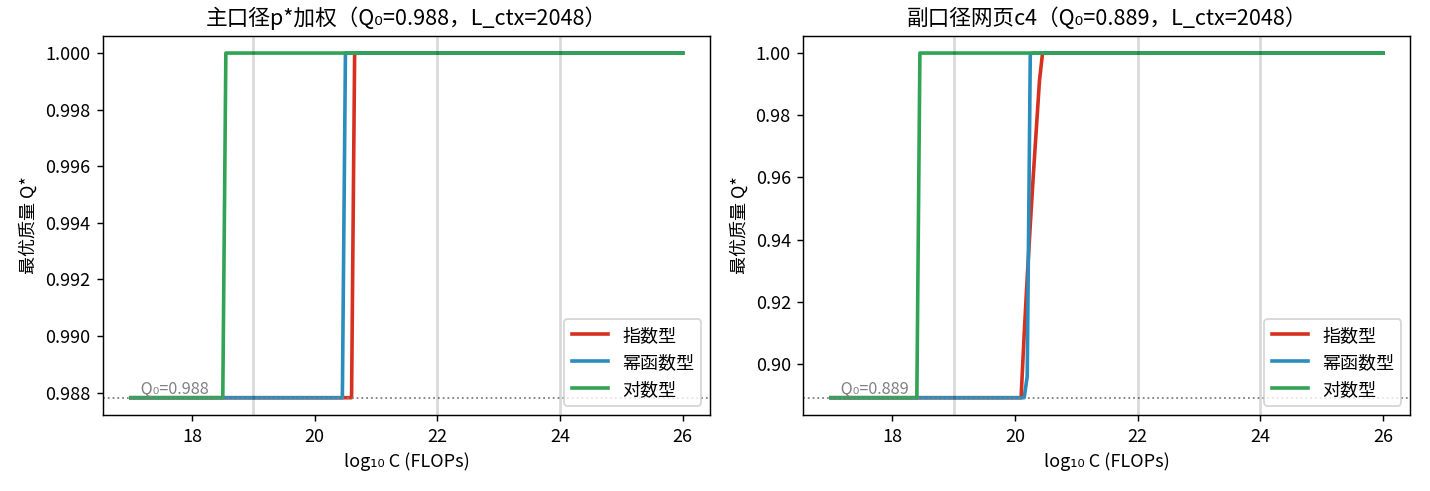
\includegraphics[width=\textwidth]{q3_F1_Qstar_vs_C.png}
\caption{最优质量 $Q^*$ 随预算的变化（三种成本函数，两种 $Q_0$ 口径）}
\label{fig:q3q}
\end{figure}

\begin{figure}[H]
\centering
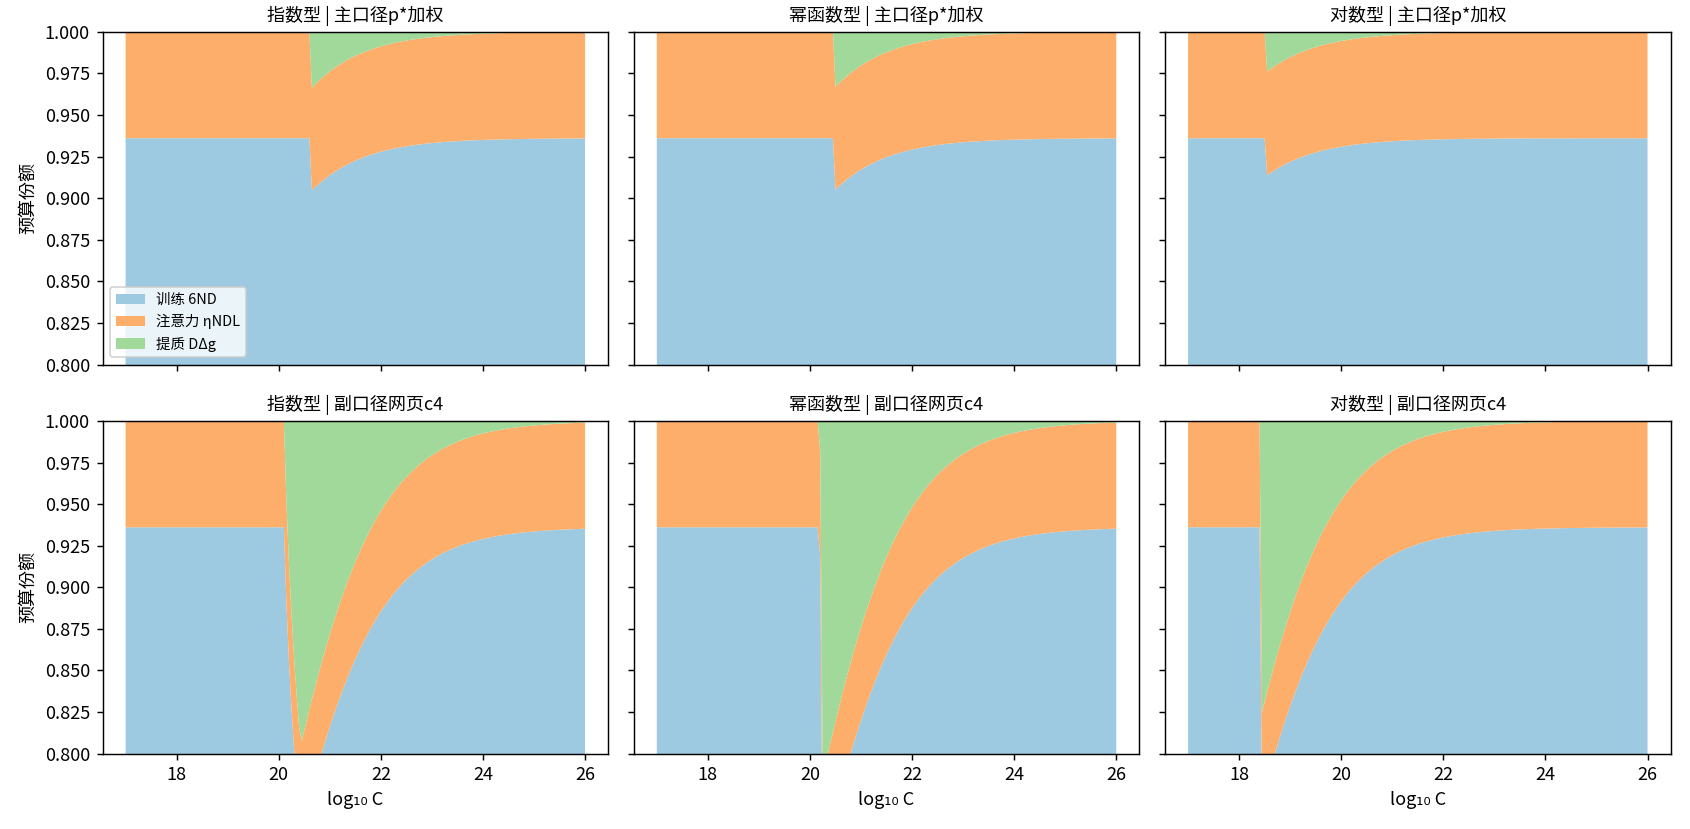
\includegraphics[width=.82\textwidth]{q3_F2_cost_shares.png}
\caption{最优解中训练、提质、注意力三项成本的占比}
\label{fig:q3share}
\end{figure}

\textbf{结构性转移。}表~\ref{tab:q3crit} 给出三种识别口径下的 $\log_{10}C_{\mathrm{crit}}$。主要发现有三点。

第一，转移几乎是跳变式的“不提质 $\to$ 提满”。主口径下“离开 $Q_0$”与“到达 $Q=1$”几乎重合（2048 档宽度 $\le0.024\dex$），原因是两个质量项对 $Q$ 都是线性的，而 $g(Q)$ 是凸的，最优解倾向落在角点。全部 210 组中有 34 组为 $Q_0$ 角点、3 组为内点，均出现在 $C=10^{19}$ 与 $10^{20}$ 的指数型与幂函数型；副口径指数型存在约 $0.33\dex$ 宽的部分提质区间。

第二，成本函数的形式决定临界点。对数型的 $g'$ 在接近 1 时最小，因此比另两种早约两个数量级开始提质。“是否提质”取决于成本函数的形式，不能一概而论。

第三，识别结果稳健。主口径三种口径的极差不超过 $0.05\dex$；副口径最大为 $0.385\dex$（指数型、$L_{\mathrm{ctx}}=131$k），仍低于事先设定的 $0.5\dex$ 一致性门槛。对问题二的 500 组 bootstrap 参数，主口径指数型 $C_{\mathrm{crit}}$ 的中位数为 $20.610$，90\% 区间为 $[20.594,20.628]$；六种组合的区间宽度都在 $\pm0.03\dex$ 以内，$10^{19}/10^{22}/10^{24}$ 三档的区制判定一致率为 100\%。

\begin{table}[H]
\centering\small
\caption{结构性转移临界预算 $\log_{10}C_{\mathrm{crit}}$（$L_{\mathrm{ctx}}=2048$）}
\label{tab:q3crit}
\begin{tabular}{llcccccc}
\toprule
$Q_0$ 口径 & $g$ & \makecell{A：离开\\$Q_0$} & \makecell{A：到达\\$Q=1$} & \makecell{A：$\Phi=1$\\解析} & \makecell{B：$s_Q$\\峰值} & \makecell{C：$D/N$\\拐点} & 极差 \\
\midrule
\multirow{3}{*}{主 0.988} & 指数型 & 20.610 & 20.634 & 20.610 & 20.65 & 20.60 & 0.050 \\
 & 幂函数型 & 20.483 & 20.483 & 20.486 & 20.50 & 20.45 & 0.050 \\
 & 对数型 & 18.523 & 18.523 & 18.540 & 18.55 & 18.50 & 0.050 \\
\midrule
\multirow{3}{*}{副 0.889} & 指数型 & 20.100 & 20.430 & 20.100 & 20.45 & 20.15 & 0.350 \\
 & 幂函数型 & 20.199 & 20.250 & 20.199 & 20.25 & 20.20 & 0.051 \\
 & 对数型 & 18.449 & 18.449 & 18.592 & 18.45 & 18.40 & 0.050 \\
\bottomrule
\end{tabular}
\end{table}

\begin{figure}[H]
\centering
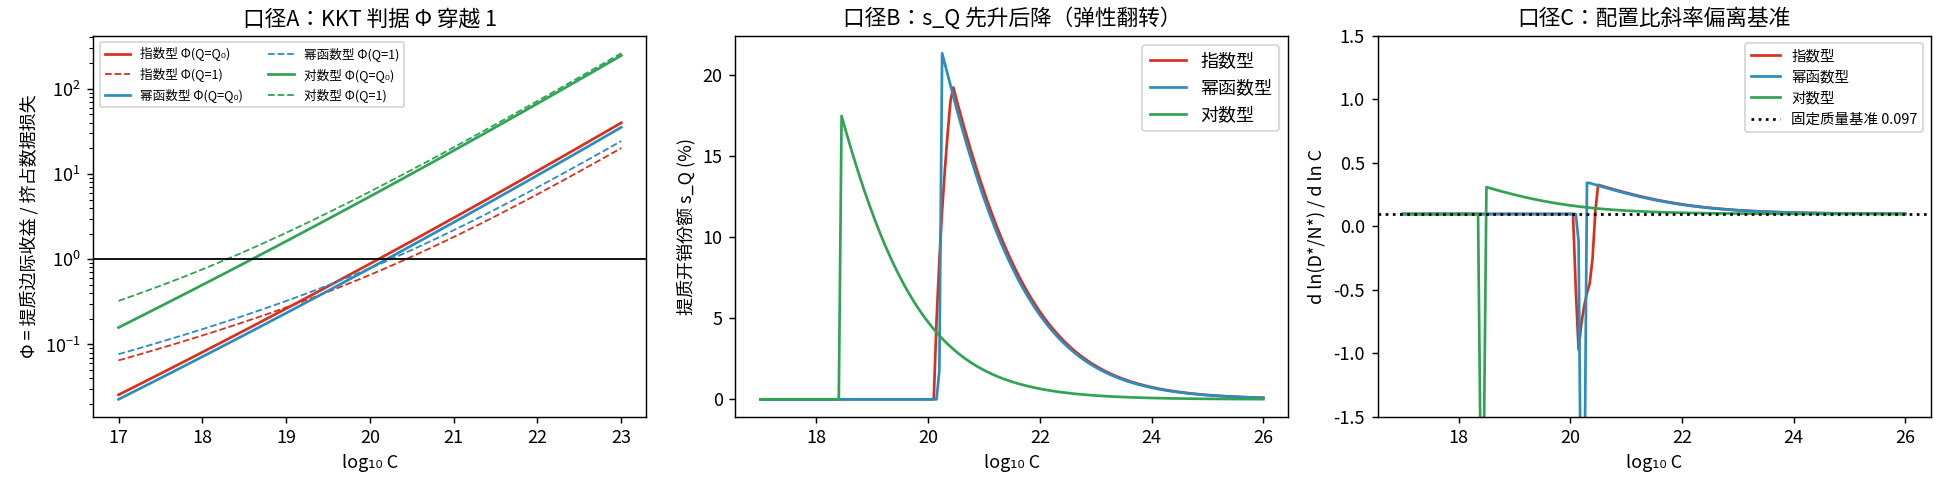
\includegraphics[width=\textwidth]{q3_F5_three_criteria.png}
\caption{结构性转移的三种识别口径（主口径）}
\label{fig:q3three}
\end{figure}

\begin{figure}[H]
\centering
\begin{minipage}{.44\textwidth}\centering
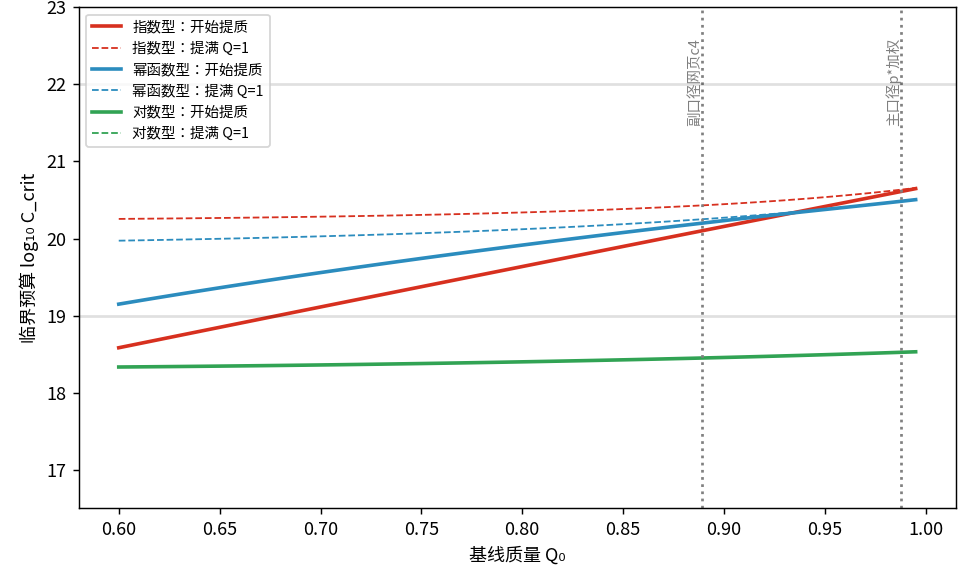
\includegraphics[width=\linewidth]{q3_F6_phase_Q0.png}
\caption{$Q_0$–$C$ 相图：$Q_0$ 越低，$C_{\mathrm{crit}}$ 越小，内点区间越宽}
\label{fig:q3phase}
\end{minipage}\hfill
\begin{minipage}{.53\textwidth}\centering
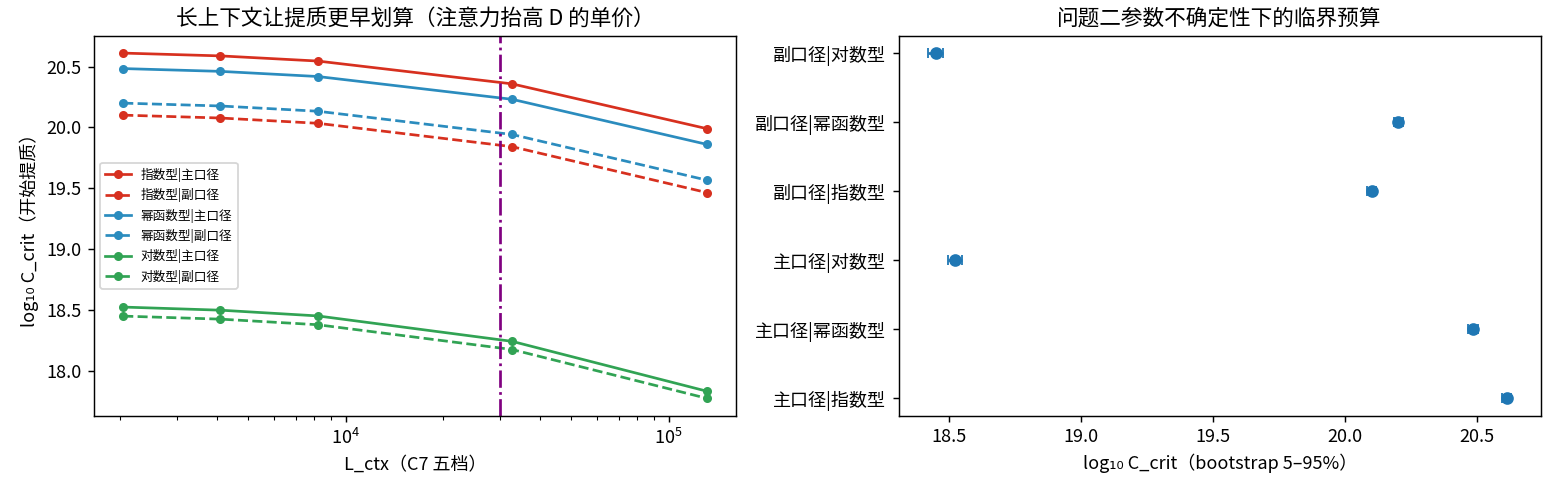
\includegraphics[width=\linewidth]{q3_F7_ccrit_sensitivity.png}
\caption{$C_{\mathrm{crit}}$ 对 bootstrap 参数与 $\eta$ 的敏感性}
\label{fig:q3sens}
\end{minipage}
\end{figure}

\textbf{上下文长度的影响。}表~\ref{tab:q3ctx} 显示，数值解与解析式 $[(6+2048\eta)/\kappa]^{0.452}$ 吻合（最大偏差 $0.002$）。32k 档刚好越过 $L_{\mathrm{ctx}}^{\mathrm{crit}}=30000$，注意力成本开始超过一半。长上下文相当于给每个参数加价，最优策略是缩小模型、按比例保留数据。$C_{\mathrm{crit}}$ 随 $L_{\mathrm{ctx}}$ 增大而单调减小（主口径指数型由 $20.61$ 降至 $19.99$），因为每 token 的训练成本变高后，同样的提质开销占比相对变小。$\eta$ 取 $\pm50\%$ 时，2048 档的 $C_{\mathrm{crit}}$ 仅移动约 $\pm0.012\dex$，131k 档移动约 $\pm0.2\dex$。

\begin{table}[H]
\centering\small
\caption{上下文长度敏感性（主口径，指数型，$C=10^{22}$）}
\label{tab:q3ctx}
\begin{tabular}{rcccccc}
\toprule
$L_{\mathrm{ctx}}$ & $\kappa$ & $N^*/N^*_{2048}$ 数值 & $N^*/N^*_{2048}$ 解析 & $L^*$ & 注意力成本占比 \\
\midrule
2\,048 & 6.41 & 1.000 & 1.000 & 2.1438 & 6.3\% \\
4\,096 & 6.82 & 0.972 & 0.972 & 2.1481 & 11.9\% \\
8\,192 & 7.64 & 0.923 & 0.924 & 2.1562 & 21.3\% \\
32\,768 & 12.55 & 0.736 & 0.738 & 2.1930 & 51.9\% \\
131\,072 & 32.21 & 0.480 & 0.482 & 2.2710 & 81.1\% \\
\bottomrule
\end{tabular}
\end{table}

\begin{figure}[H]
\centering
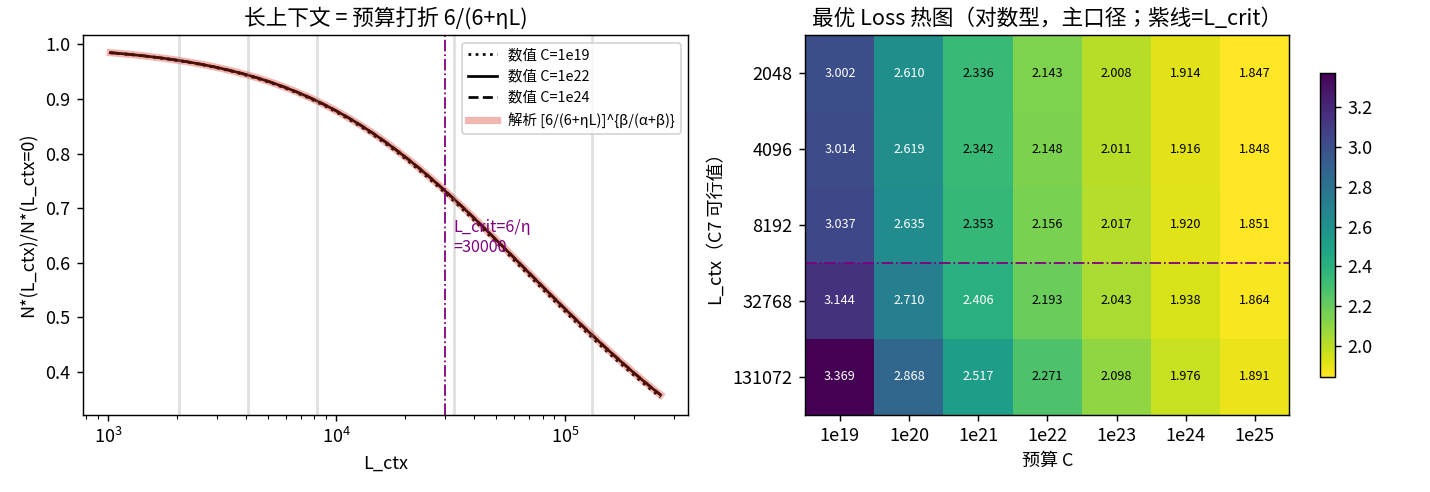
\includegraphics[width=\textwidth]{q3_F4_Lctx_sensitivity.png}
\caption{$L_{\mathrm{ctx}}$ 对最优规模、$C_{\mathrm{crit}}$ 与成本结构的影响}
\label{fig:q3ctx}
\end{figure}

\textbf{配比联立。}把配比也纳入决策，联合目标为 $L_{\mathrm{joint}}=L(N,D,Q)\cdot m(\bp)$。其中 $m(\bp)$ 用问题一求 $\bp^*$ 时的同一组 13 个验证域梯度提升模型计算，并以 $\bp^*$ 处为 1 归一化；提质起点改为 $Q_0(\bp)=\sum_ip_iQ_{\mathrm B,i}$；在 $\bp^*$ 周围做 Dirichlet 采样，共 4000 个候选。结果显示，联合最优相对 $\bp^*$ 可再降 $13.69\%$–$13.78\%$，其中配比效应 $1-m$ 贡献 $13.69\%$，规模与提质通道只贡献 $0.001\%$–$0.105\%$。若取最优前 100 个点的平均，与 $\bp^*$ 的全变差距离为 $0.017$–$0.022$，收益为 $1.0\%$–$2.2\%$，更为稳健。在不同 $(g,C)$ 组合下，4000 个候选的排序秩相关最小为 $0.976$（图~\ref{fig:q3mix}）。因此配比决策与规模/质量决策近似可分离，“先定配比、再定规模”的做法成立。

\begin{figure}[H]
\centering
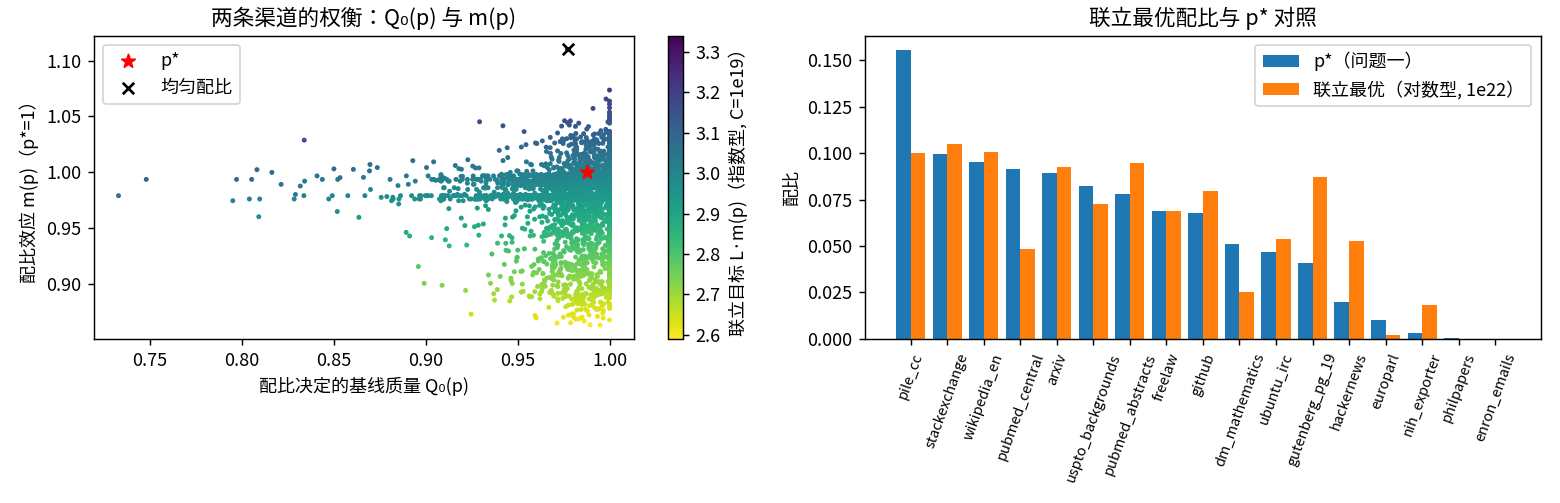
\includegraphics[width=\textwidth]{q3_F8_mixture_joint.png}
\caption{配比联立优化：降损来源分解与跨预算排序一致性}
\label{fig:q3mix}
\end{figure}

\textbf{对《数据说明》中建议的核对。}说明文档称“$C=10^{22}$ 时 $N^*=1.2\times10^{-3}$B、$D^*=850$B、Loss $=3.41$”。该配置只用掉 $0.06\%$ 的预算，按本文标度律其损失为 $5.361$，而真实最优为 $L^*=2.143$、$N^*\approx5\times10^9$。说明文档称“各档预算 $Q^*=1$，无需比较成本函数”，与上文 34 组 $Q_0$ 角点 + 3 组内点的结果矛盾。说明文档建议“穷举网格 + 罚系数取 1”，但由式~\eqref{eq:dsolve} 可解析消去约束；网格法与本文求解器的 Loss 差虽不超过 $1.6\times10^{-5}$，却无法连续识别 $C_{\mathrm{crit}}$。

\subsection{问题四的模型建立与求解}

\subsubsection{模型建立}

\textbf{四项口径。}赛题要求逐条说明的四项口径见表~\ref{tab:q4kou}。按许可证分档后，permissive 与 community 两档的 base 前沿（Top-5 Average 均值）几乎持平（$34.24$ 与 $33.60$），noncommercial 档样本少、前沿偏低（$9.58$）。因此“开源前沿”取全部可下载权重的模型，不再按许可证剔除。

\begin{table}[H]
\centering\small
\caption{问题四的四项口径}
\label{tab:q4kou}
\begin{tabular}{p{1.9cm}p{6.4cm}p{6.1cm}}
\toprule
口径 & 主口径 & 副口径 / 说明 \\
\midrule
能力度量 & C1 Average（六维等权，已扣随机基线，0–100） & C8 逐任务重算的去饱和综合分 \\
开源筛选 & C1/C2 均来自 HF Hub，权重可下载；按许可证分三档 & C4 中 Model accessibility 含 Open weights（1961 个 LM 中 901 个） \\
模型类型 & base = pretrained 275 + continuously pretrained 58 = 333 & chat = chat 718 + fine-tuned 1785 = 2503；merges / multimodal 剔除 \\
时间轴 & C2 真实发布日（447 行有值） & C1 提交日中位滞后 103.5 天，只用于月度窗口与回测 \\
\bottomrule
\end{tabular}
\end{table}

\textbf{任务饱和与去饱和分。}C8 的每个叶子任务按随机基线归一化，$\hat s=\max\{0,(s-c)/(1-c)\}$，其中 $c$ 为随机猜测得分。月度累计前沿按“终点前沿、剩余空间、关闭率、噪声门槛”四个判据，把 39 个任务分为饱和、快速增长、常规增长、低位停滞四类。去饱和综合分剔除饱和任务，其余任务按起点剩余空间加权、各 family 等权。

\textbf{Loss–Benchmark 桥接。}得分有底噪下界和上界，因此采用 S 形映射
\begin{equation}
S=lo+\frac{hi-lo}{1+e^{\,k(L-L_0)}} ,
\label{eq:bridge}
\end{equation}
给定 $(k,L_0)$ 时 $(lo,hi)$ 可线性求解。C6 按可比性分层：High 层（Pythia，同模型同验证集，7 条）权重 1；Medium 层（不同验证集，近似可比，68 条）权重 0.5。High 层的 Val\_Loss 与问题二标度律 $\hat L$ 的差小于 $10^{-4}$，证明二者处于同一尺度。

\textbf{分解模型。}以问题二标度律（$Q=1$）计算每个模型的 $\hat L(N,D)$，作为“规模状态”。主模型（M1b，结构·加性）为
\begin{equation}
S_m=lo+amp\cdot\sigma\bigl(k(\hat L_m-L_0)\bigr)+\tau\,(t_m-2023)+\varepsilon_m,
\label{eq:m1b}
\end{equation}
其中 $\sigma$ 为 logistic 函数。$\tau$ 是每年的得分技术增益，也就是“非规模技术进步”。副模型 M1c 把技术项写成等效降损，$\sigma\bigl(k(\hat L_m-\delta t_m-L_0)\bigr)$。对照模型包括：M2 效率前沿（Epoch 口径，帕累托有效模型上的 $S=a+b\log_{10}C+ct$）、M3 分位数回归与全样本 OLS。前沿增量用 Shapley 值分解（两种顺序的平均）：“规模贡献”为只让前沿 $\hat L$ 按实际演进时的增量，“技术贡献”为只让 $t$ 演进时的增量。

\textbf{预测链条。}预测不新增自由参数，四步依次为：算力情景 $\to$ 问题三最优配置（$Q=1$，$L_{\mathrm{ctx}}=4096$）下的 $\Delta L^*$ $\to$ 叠加到前沿 $\hat L$ 上（锚定增量：现有前沿并非算力最优，只借用 $L^*$ 的斜率）$\to$ 经式~\eqref{eq:m1b} 与技术项得到 $\Delta S$。chat 前沿等于 chat 锚点加上 base 增量，再加上后训练增益增量。

\subsubsection{求解方法}

C8 共 1958 个 JSON，逐任务解析；重算的六个 family 分与 C1 的 Pearson 相关 $\ge0.989$（MATH 为 $0.801$），说明解析口径正确。式~\eqref{eq:bridge} 采用“网格 + 两级加密 + 加权最小二乘”拟合（环境无 scipy），用留一交叉验证比较 sigmoid、线性与常数三种桥接。分解面板由 C2 与 C4 按（发布日，组织）联表得到：base 58 行，其中 23 行的 $D$ 由 $C/(6N)$ 反解；chat 37 行，只保留同时发布了 base 的原厂组织。区间由模型簇重抽样 bootstrap（120 次）给出。预测部分做 4000 次蒙特卡洛，不确定性来源依次为：问题二 bootstrap 参数，分解 bootstrap（M1b 与 M1c 各半），后训练增益 bootstrap，前沿残差（sd $2.05$）。回测只用 $t<2024.5$ 的数据重估模型，再预测 2025.25 的前沿。

\subsubsection{结果与分析}

\textbf{任务饱和。}39 个任务中 10 个饱和（temporal\_sequences 达到 $1.00$，另有 IFEval、hyperbaton 等），9 个快速增长（web\_of\_lies 由 $0.20$ 升至 $0.78$），17 个常规增长，3 个低位停滞（gpqa\_diamond 等）。表~\ref{tab:q4desat} 显示，模型级去饱和分与 Average 的相关为 $0.948$，排序基本一致，但饱和任务稀释了增速：按相对增幅计，Average 低估前沿进展约 $1.6$ 倍。

\begin{table}[H]
\centering\small
\caption{三种能力口径下的前沿变化（C1 提交日窗口）}
\label{tab:q4desat}
\begin{tabular}{lcccc}
\toprule
口径 & 2024-06 前沿 & 2025-03 前沿 & 相对增幅 & 月斜率 \\
\midrule
C1 Average & 38.52 & 49.89 & $+29.5\%$ & 1.285 \\
C8 全任务重算 & 37.98 & 49.40 & $+30.1\%$ & 1.326 \\
\textbf{C8 去饱和分} & 26.36 & 39.06 & $\mathbf{+48.2\%}$ & 1.536 \\
\bottomrule
\end{tabular}
\end{table}

\begin{figure}[H]
\centering
\begin{minipage}{.5\textwidth}\centering
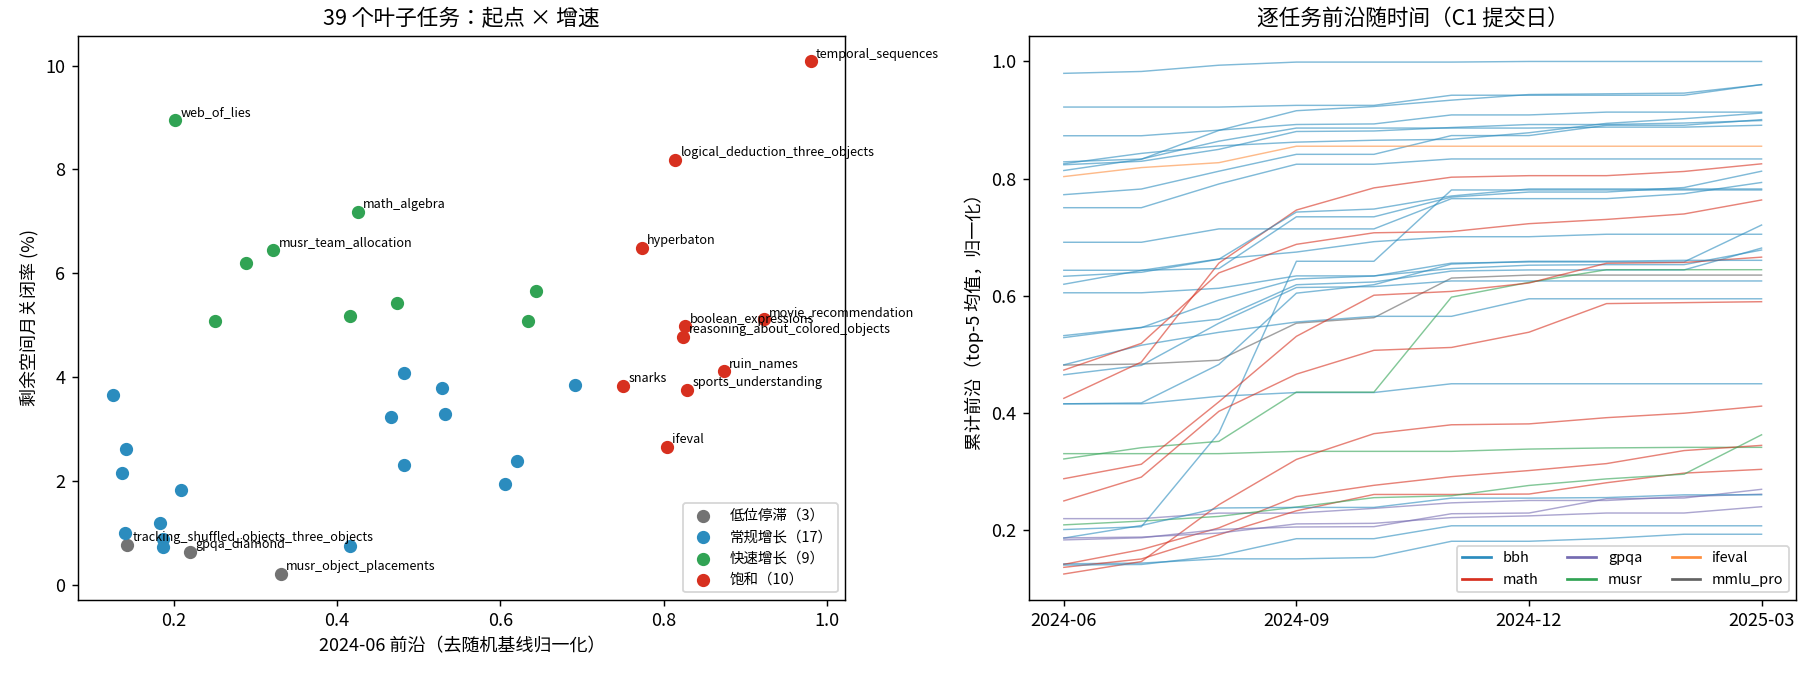
\includegraphics[width=\linewidth]{q4_F9_task_saturation.png}
\caption{39 个叶子任务的饱和度分类}
\label{fig:q4sat}
\end{minipage}\hfill
\begin{minipage}{.47\textwidth}\centering
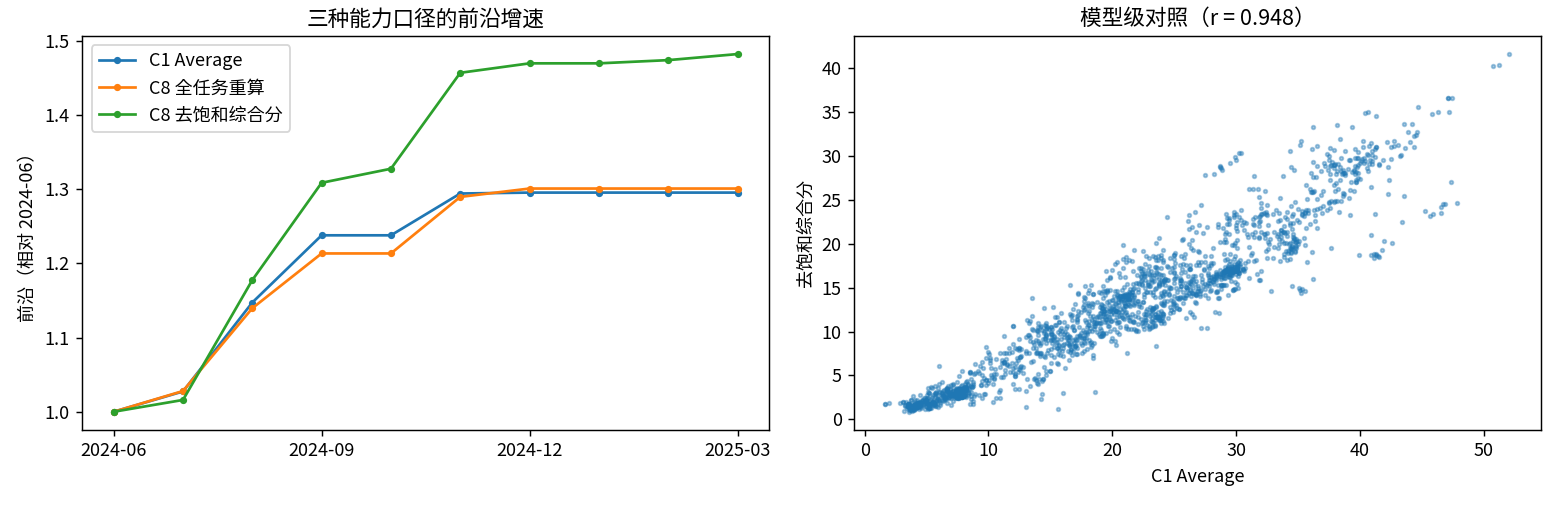
\includegraphics[width=\linewidth]{q4_F10_desat_vs_avg.png}
\caption{去饱和分与 Average 的前沿对比}
\label{fig:q4desat}
\end{minipage}
\end{figure}

\textbf{桥接。}Loss 与 Average 负相关：全体 $r=-0.510$，High 层 $-0.397$，Medium 层 $-0.502$。base 主桥接为 $lo=8.63$、$hi=21.57$、$k=46.1$、$L_0=2.07$。留一 RMSE 为：sigmoid $8.08$、线性 $8.28$、常数 $9.51$。只用系列内变异的固定效应斜率为 $dS/dL=-23.6$（base）与 $-36.7$（chat）。Medium 层权重取 $0.25/0.5/1.0$ 时，$S(L=1.85)$ 分别为 $21.79/21.57/21.43$，结果稳定。但 High 层的 7 个点全部落在底噪区（$L\in[2.09,2.60]$），只能锁定下界，S 形的上升段依赖 Medium 层，这是 C6 数据的硬限制。

\begin{figure}[H]
\centering
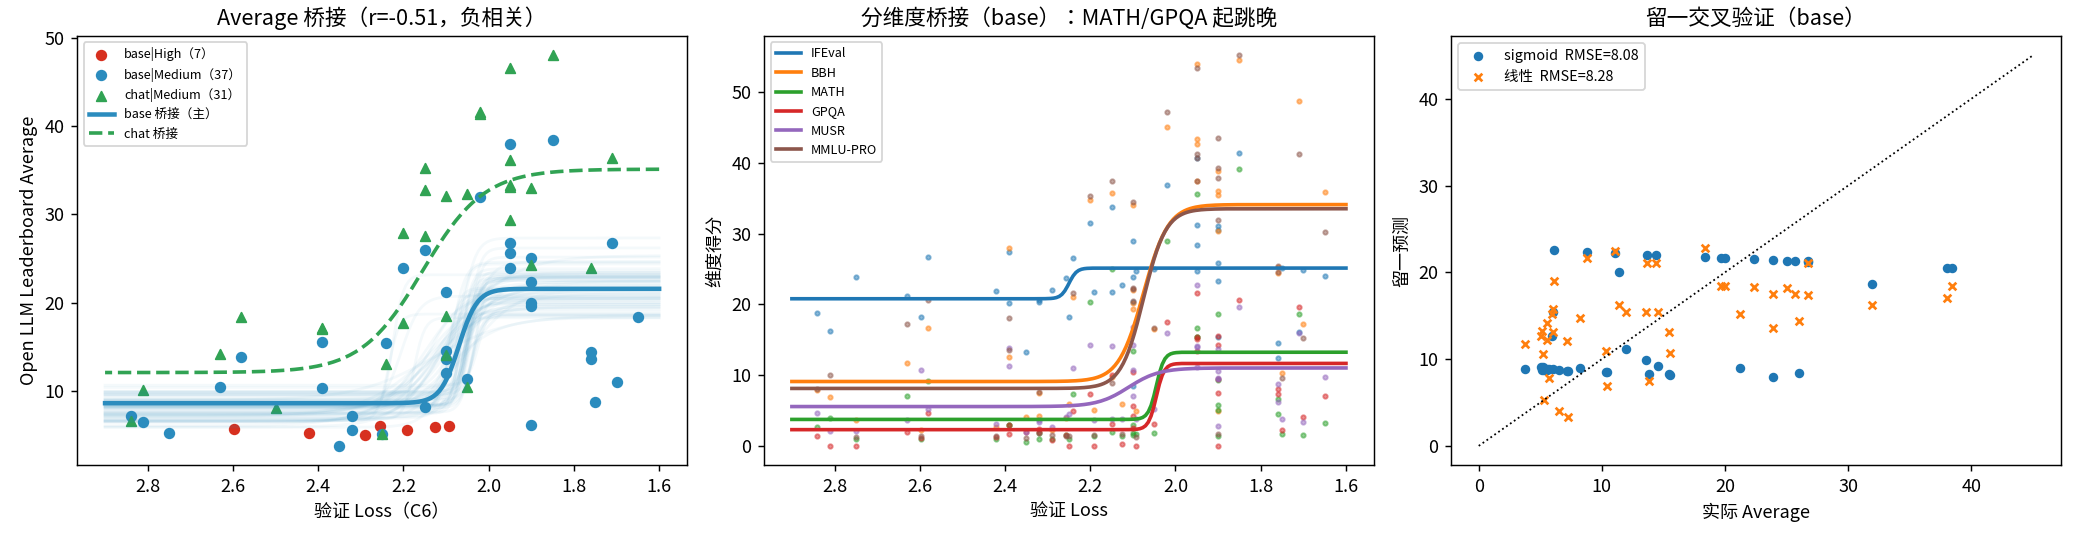
\includegraphics[width=\textwidth]{q4_F11_bridge.png}
\caption{C6 分层 Loss–Benchmark 桥接（base 与 chat）}
\label{fig:q4bridge}
\end{figure}

\textbf{贡献分解。}主模型 M1b 的估计为 $\tau=2.45$ 分/年，$R^2=0.870$；去掉 $\tau$ 后 $R^2$ 降为 $0.832$；M1c 的 $\delta=0.035$ Loss/年。主窗口 2023.5$\to$2025.0 内，base 前沿由 $12.54$ 升至 $37.30$（$\Delta S=24.76$），$\hat L$ 由 $2.006$ 降至 $1.869$，$\log_{10}C$ 由 $23.35$ 升至 $24.64$。表~\ref{tab:q4decomp} 给出各方法的分解结果。

\begin{table}[H]
\centering\small
\caption{base 前沿增长的贡献分解（2023.5$\to$2025.0，Shapley）}
\label{tab:q4decomp}
\begin{tabular}{llcccc}
\toprule
类别 & 方法 & 规模贡献 & 技术贡献 & 技术占比 & 90\% 区间 \\
\midrule
\multirow{2}{*}{结构模型} & \textbf{M1b（主）} & 23.06 & 3.40 & \textbf{12.9\%} & 6\%–22\% \\
 & M1c & 20.12 & 6.04 & 23.1\% & 4\%–46\% \\
\midrule
\multirow{4}{*}{线性对照} & M2 效率前沿 & 7.36 & 6.19 & 45.7\% & 9\%–60\% \\
 & M3 $q=0.75$ & 7.40 & 4.45 & 37.5\% & — \\
 & M3 $q=0.5$ & 6.24 & 5.88 & 48.5\% & — \\
 & OLS & 7.72 & 3.24 & 29.5\% & — \\
\midrule
反例 & M1a 桥接直接套用 & 0.63 & 4.84 & 88\% & 不可迁移 \\
\bottomrule
\end{tabular}
\end{table}

核心三法（M1b、M2、M3 $q=0.75$）的极差为 $32.8$ 个百分点，超过事先设定的 $\pm15$pp 一致性门槛，因此不强行给出单一数字。差异是结构性的：M2 与 M3 假设得分对 $\log C$ 线性，无法表达桥接的 S 形加速段，把“Loss 刚进入陡峭区带来的规模红利”部分记到了时间项上；M1b 与 M1c 用“标度律 + S 形桥接”吸收了这部分，拟合优度也明显更高（$R^2$ $0.87$ 对 $0.66$）。故主结论采用结构口径：\textbf{规模扩张贡献约 77\%–87\%，非规模技术进步约 13\%–23\%}；线性口径的 30\%–46\% 作为上界参考。所有方法在“规模为主”这一定性结论上一致。M1a 直接套用 C6 桥接（$hi=21.6$，低于面板前沿），把桥接的非线性全部记为“技术”，得到 88\%，与索洛余值法的偏差同源，只作为反例列出。

换算为算力等效，各方法的技术进步为：M1b $0.29$、M1c $0.56$、M2 $0.78$、OLS $0.39\dex/\mathrm{yr}$。这与 C1 窗口内回归的 $0.44$–$0.77\dex/\mathrm{yr}$ 同量级，两者相互印证。加入 C3 历史点做敏感性：权重 $0.2$ 时为 $0.50\dex/\mathrm{yr}$。C3 的 Average 与其六维均值的相关仅为 $0.634$，口径混杂，因此不进入主结果。

\textbf{chat 与后训练。}在 89 对同组织的 (base, chat) 配对中，后训练平均增益为 $4.30$ 分；对有发布日的 31 对做回归，得 $G(t)=-0.40+3.35\,(t-2023)$，说明后训练本身是一类逐年增强的非规模技术。chat 前沿在 2023.5$\to$2025.0 由 $8.76$ 升至 $46.06$：规模贡献 $23.77$，预训练技术 $3.56$，后训练技术 $4.86$，技术占比 $26\%$。

\begin{figure}[H]
\centering
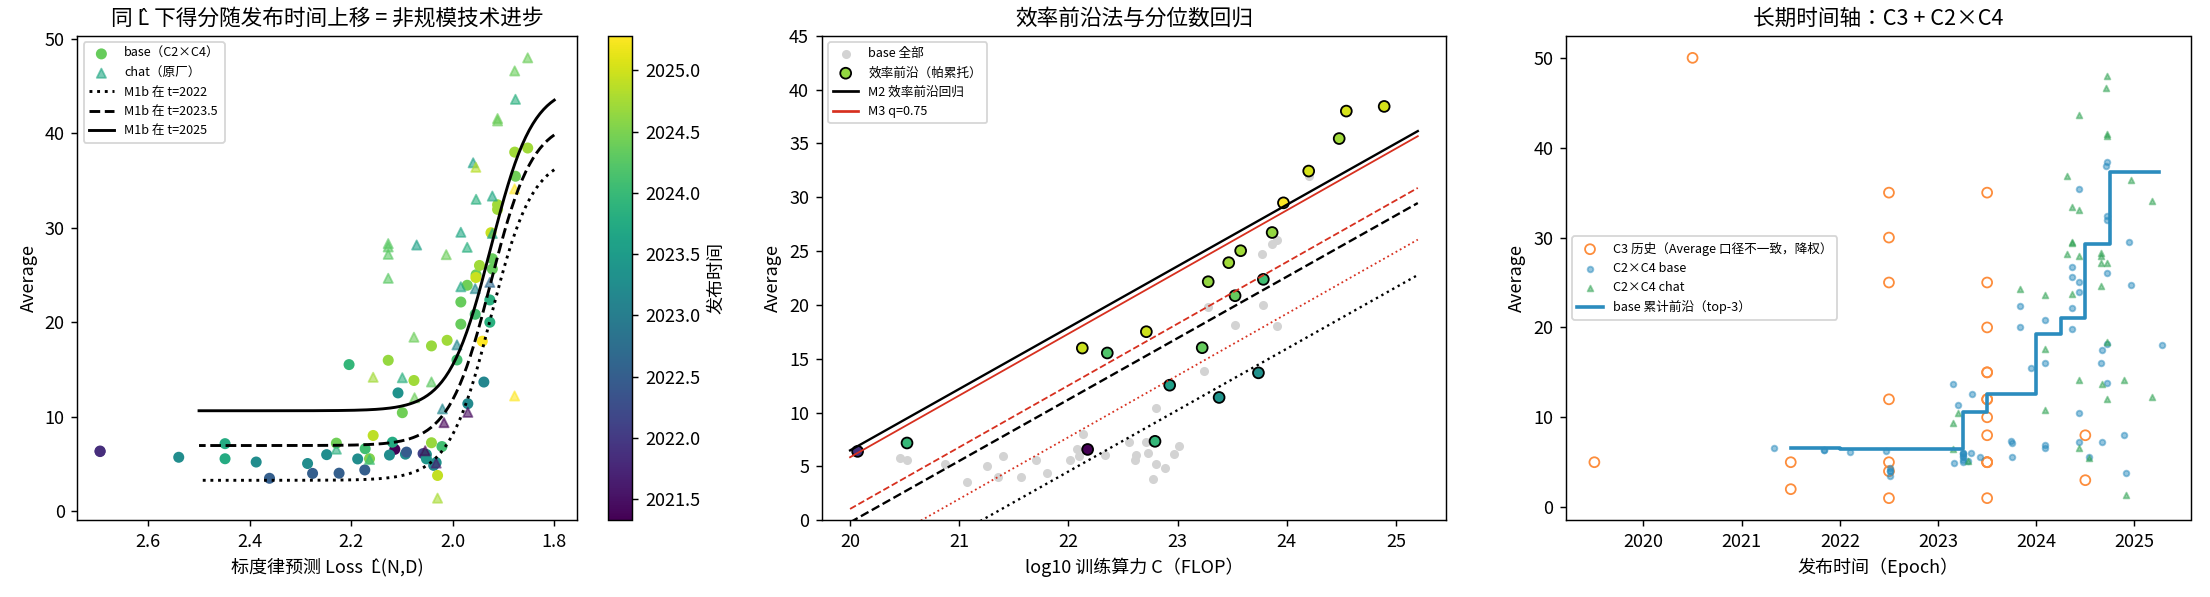
\includegraphics[width=\textwidth]{q4_F12_decomp_panel.png}
\caption{分解面板：规模状态 $\hat L$、得分与时间}
\label{fig:q4panel}
\end{figure}

\begin{figure}[H]
\centering
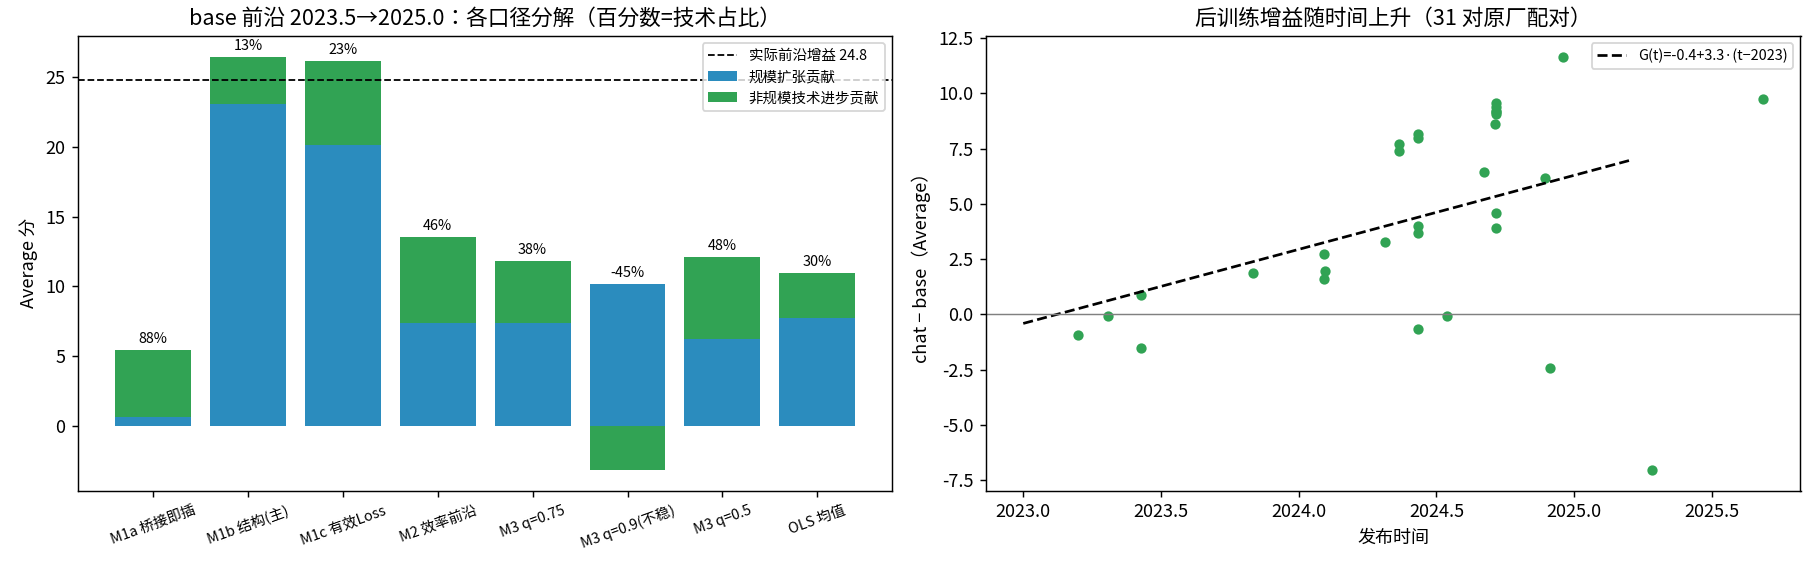
\includegraphics[width=.9\textwidth]{q4_F13_decomp_bars.png}
\caption{各方法、各窗口的规模/技术贡献}
\label{fig:q4bars}
\end{figure}

\textbf{算力放缓情景与前沿预测。}C4 中开源权重模型的年度最大训练算力，2019 年为 $10^{22.52}$，2025 年为 $10^{25.59}$。按最大值、Top-5、2022–25 与全部 LM 四种统计，斜率分别为 $0.58/0.60/0.69/0.65\dex/\mathrm{yr}$。据此设三种情景：基线 $0.60$、减半 $0.30$、1/4 $0.15\dex/\mathrm{yr}$。起点 $T_0=2025.25$，锚点 base $S=37.30$（$\hat L=1.869$），chat $S=46.06$。预测结果见表~\ref{tab:q4fc}。

\begin{table}[H]
\centering\small
\caption{开源前沿（Average）预测：中位数 [90\% 区间]}
\label{tab:q4fc}
\begin{tabular}{lccccc}
\toprule
\multirow{2}{*}{情景} & \multicolumn{3}{c}{base} & \multicolumn{2}{c}{chat（24 个月）} \\
\cmidrule(lr){2-4}\cmidrule(lr){5-6}
 & 12 个月 & 24 个月 & 技术占比 & 后训练增益延续 & 后训练增益停滞 \\
\midrule
基线 0.60 & 43.1 [37.4, 52.8] & 46.2 [37.5, 68.5] & 55\% & 61.6 [51.8, 79.6] & 54.8 [46.4, 70.1] \\
减半 0.30 & 41.7 [37.0, 49.7] & 45.2 [37.7, 58.3] & 65\% & 60.7 [51.5, 75.3] & 54.0 [46.2, 67.6] \\
1/4\ \ 0.15 & 41.1 [36.6, 47.6] & 44.1 [37.5, 54.9] & 77\% & 59.8 [50.9, 71.6] & 52.7 [46.1, 63.3] \\
\bottomrule
\end{tabular}
\end{table}

算力增速从 $0.60$ 降到 $0.15\dex/\mathrm{yr}$，24 个月的 base 中位数只减少约 2 分（$46.2\to44.1$）。原因是规模增量本身被 S 形桥接的饱和段压缩（规模部分由 $3.9$ 分降为 $1.5$ 分），而技术项（约 5 分）基本不受影响。所以\textbf{算力放缓时，技术进步成为增量主体}（占比由 55\% 升至 77\%）。模型不确定性主要来自技术项的形式：基线情景下 M1b 的中位数为 $46.6$，M1c 为 $44.7$，后者上尾更宽。chat 前沿对“后训练增益是否延续”最敏感（相差约 7 分），这一差别大于算力情景之间的差别（约 2 分）。作为上界参考，M1b 的纯规模天花板为 $44.2$，“算力无限”时 24 个月为 $49.2$。

\begin{figure}[H]
\centering
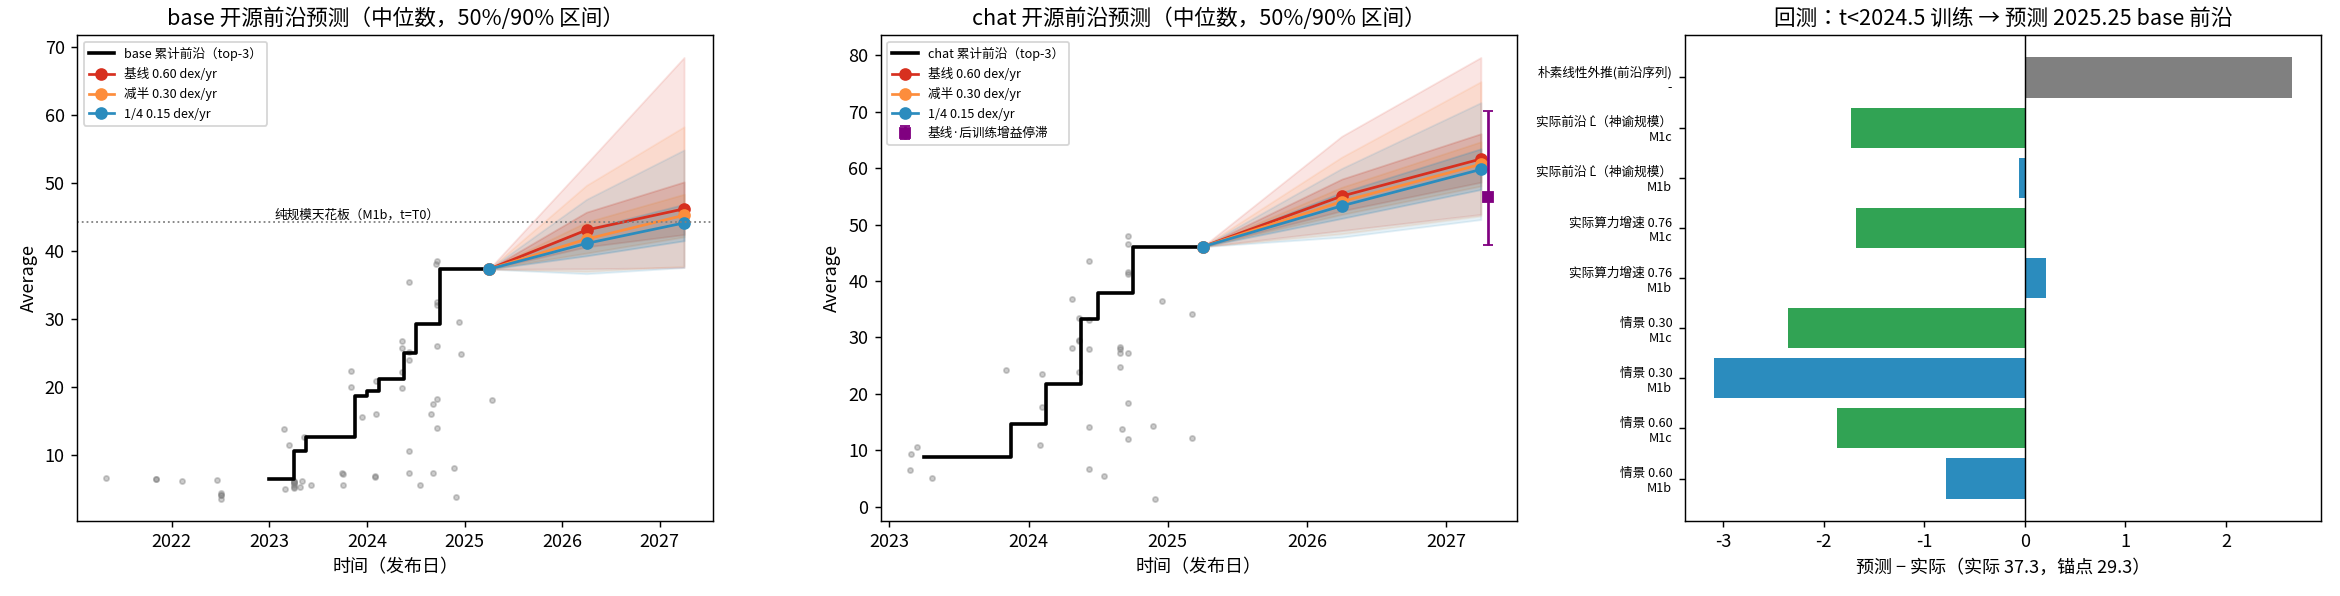
\includegraphics[width=\textwidth]{q4_F14_forecast.png}
\caption{三种算力情景下 base/chat 开源前沿的 12/24 个月预测（阴影为 90\% 区间）}
\label{fig:q4fc}
\end{figure}

\textbf{回测。}只用 $t<2024.5$ 的 42 个 base 模型重估模型（$\tau=2.74$），以 2024.5 的前沿 $29.28$ 为锚点，预测 2025.25 的前沿（实际为 $37.30$）。M1b 在基线情景下的误差为 $-0.78$，用实际算力增速（$0.76\dex/\mathrm{yr}$）时误差为 $+0.21$，朴素线性外推的误差为 $+2.65$。在提交日轴上，C1 月度前沿做纯时间序列外推，3 个月误差达到 $+7.91$，因为前沿在 $49.89$ 附近进入平台。这是不直接用 ARIMA 外推的实证理由。

\textbf{对《数据说明》中建议的核对。}(i) 说明文档称“Loss–Benchmark 正相关 $r=+0.68$”，实测为 $r=-0.51$。(ii) 说明文档称“$b_N=-6.2$，规模越大得分越低”，实测规模系数全部为正（C1 窗口 $7.41$，面板 $6.85$，效率前沿 $5.71$）。(iii) 说明文档建议“年份独热编码”，但独热编码无法外推到未见年份，本文改用连续时间项，并以算力等效率互证。(iv) 索洛余值法把桥接的非线性全部记入技术项（即 M1a 的 88\%），本文把它列为反例，并用结构模型修正。

\section{模型的检验与灵敏度分析}

\subsection{模型检验}

表~\ref{tab:checks} 汇总了全文的检验。“互相验证”只用于\emph{同一问题、不同假设}的方法对，判据取排序或数值的一致性；上下游分工衔接的方法之间不存在验证关系，本文也不作此类声称。

\begin{table}[!htbp]
\centering\small
\caption{全文检验清单}
\label{tab:checks}
\setlength{\tabcolsep}{3pt}
\begin{tabular}{cp{4.3cm}p{2.2cm}p{2.8cm}p{4.3cm}}
\toprule
问题 & 检验对 & 类型 & 判据 & 结果 \\
\midrule
\multirow{6}{*}{一}
& CRITIC--Huber vs 加权均值/PCA/TOPSIS & 方法一致性 & 样本级 Spearman & $0.9936/0.8166/0.9588$ \\
& A1 对 A2/A3 对应域全量 & 分布比较 & KS 检验 & arxiv/github：$p=0.313/0.220$ \\
& 六来源分歧诊断 & 冻结规则复检 & 候选比例 & 高分歧：$5.00\%/4.73\%/4.99\%$；多来源对立：$1.36\%/1.58\%/1.77\%$ \\
& clr+Huber / 裸 OLS / GBDT & 1M 留出集拟合 & 平均逐域 $R^2$ & $0.772/0.654/0.897$ \\
& 配比质量交互 & bootstrap 稳健性 & 区间不含零的域数 & $6/13$，系数正负并存 \\
& 1M $\to$ 60M $\to$ 1B & 冻结模型检验 & 排名 Spearman；$R^2$ & $0.523/0.467/0.677$；$0.772/-7.69/-604.66$ \\
\midrule
\multirow{3}{*}{二}
& B6 拟合 / B7 新增点 & 半合成留出检验 & RMSE & $0.0515/0.0416$ \\
& B7 仿射形状（全 450 点） & 形状检查，非独立检验 & $R^2$；二次项 $t$ & $0.9974$；$-0.35$ \\
& B4/B5 对经典基线 & 跨来源趋势对照 & Spearman & $0.983/0.959$；仅检验经典 $N,D$ 趋势 \\
\midrule
\multirow{3}{*}{三}
& 数值解 vs 闭式 $N^*$ & 互相验证 & 相对误差 & $\le1.83\times10^{-7}$（15 组） \\
& 求解器 vs 网格穷举 & 互相验证 & Loss 差、区制 & $\le1.6\times10^{-5}$，区制一致 \\
& $C_{\mathrm{crit}}$ 三口径 & 互相验证 & 极差 & 主口径 $\le0.05\dex$ \\
\midrule
\multirow{4}{*}{四}
& C8 重算 vs C1 & 口径核验 & Pearson & $\ge0.989$（MATH $0.801$） \\
& sigmoid vs 线性桥接 & 形式选择 & 留一 RMSE & $8.08$ vs $8.28$ \\
& 分解 dex/yr vs 窗口回归 & 互相验证 & 同量级 & $0.29$–$0.78$ vs $0.44$–$0.77$ \\
& 预测回测 & 外部检验 & 2025.25 误差 & M1b $-0.78$，线性外推 $+2.65$ \\
\bottomrule
\end{tabular}
\end{table}

不一致的地方同样是结论。问题一的 17 域质量与训练边际价值秩相关为 $-0.211$，只能说明样本内关联较弱，不能据此推断质量与训练价值完全无关；60M/1B 的配比排序相关仍为正，但绝对损失拟合的 $R^2$ 显著为负，不能把排序保持说成绝对预测有效；问题四中结构模型与线性模型相差 32.8pp，本文如实并列，并解释其来源。A12–A15、B6–B8 与 B10 的证据等级（估算/外推、半合成）在全文中始终保留标注，没有升格为实证。

\subsection{灵敏度与稳健性分析}

\textbf{问题一。}六来源候选比例的操作阈值由 A1 每域的 $B(x)$ 第 95 百分位确定，A2/A3 冻结复用。固定高低端立场为两端 20\% 时，阈值改为 P90/P95/P97.5，A1 候选比例为 $10.00\%/5.00\%/2.50\%$，A2 为 $9.19\%/4.73\%/2.00\%$，A3 为 $9.74\%/4.99\%/2.44\%$；筛查比例随操作点变化，不代表真实冲突发生率。当前无人工质量真值，诊断结果未用于更新主 $Q$。等权与 pile\_cc 单域目标分别搜索配比，因目标不同而得到不同候选份额。

\textbf{问题二。}按 B6 拟合的修订质量律参数为 $\kappa_N=0.4297,\kappa_D=0.1395,k_0=0.1417$；B7 新增 90 个半合成点的留出 RMSE 为 $0.0416$。A、B 质量映射采用 $Q_B=Q_A$ 作为条件性主锚点，当前问题一等权目标质量为 $0.6609$；锚点尚未由损失数据识别，质量项区间估计和锚点敏感性仍待补齐。按式~\eqref{eq:sub} 推导的等效替代关系仅是半合成模型内的解析结论。

\textbf{问题三。}对问题二的 500 组 bootstrap 参数，$C_{\mathrm{crit}}$ 的区间宽度在 $\pm0.03\dex$ 以内。$\eta$ 取 $\pm50\%$ 时，2048 档的 $C_{\mathrm{crit}}$ 移动约 $\pm0.012\dex$，131k 档移动约 $\pm0.2\dex$，此时 $L_{\mathrm{ctx}}^{\mathrm{crit}}$ 相应变为 $60000/20000$。$Q_0$ 相图（图~\ref{fig:q3phase}）表明：$Q_0$ 越低，$C_{\mathrm{crit}}$ 越小，内点区间越宽。

\textbf{问题四。}C6 中 Medium 层的权重取 $0.25$–$1.0$ 时，$S(1.85)$ 的变化不到 $0.4$ 分。C3 历史点的权重取 $0.2$ 与 $1.0$ 时，技术进步率分别为 $0.50$ 与 $0.21\dex/\mathrm{yr}$，因此只作敏感性分析。分解换用 2024$\to$2025 与 2024.5$\to$2025.25 两个窗口，M1b 的技术占比为 $7.1\%$ 与 $8.2\%$，M2 为 $30.6\%$ 与 $24.3\%$，“规模为主”的定性结论不变。

\section{模型的评价与推广}

\subsection{模型的优点}

(1) \textbf{证据分层。}半合成与外推数据分别标注其性质和适用边界；问题一的估算表只用于跨尺度敏感性讨论，问题二以 B1 校准、B6 拟合并用 B7 新增点留出检验质量项。

(2) \textbf{口径可追溯。}Q1 的指标方向、归一化、CRITIC 权重和 Huber 阈值均由 A1 拟合并冻结；六来源冲突诊断分别报告来源内与来源间差异，阈值对应明确的筛查预算；配比模型通过留出集比较，结构性转移由 KKT 活跃集定义。

(3) \textbf{解析表达与数值核验。}问题二旧版的四条命题曾与旧求解器数值逐项对照；本轮修订质量律已推导边际效应、替代条件与算力最优式，但对应数值表尚未重算互验。问题三、四的旧接口数值也须待跨问同步后复核。

(4) \textbf{区分评分与诊断。}质量评分给出唯一主分，六来源冲突分析只用于揭示信号分歧和形成复核候选；没有把筛查比例写成真实冲突率，也没有把评分稳健性证据解释成质量准确率。

\subsection{模型的局限与改进方向}

(1) 11 个 inferred 域的质量分依赖桥接函数（五折 $R^2_{\mathrm{cv}}=0.4106$），区间未纳入模型选择及跨域偏差；六个映射域的验证样本数也有限。若能增补这些域的直接质量信号，可进一步检验桥接假设。

(2) 问题一尚无独立人工质量真值；CRITIC--Huber 与其他排序的一致性、极端指标剔除实验和冲突候选复检都不能替代准确性验证。诊断后的人工复核处置与模型更新尚未完成。

(3) 本轮问题一主质量分和领域分已更新；问题二的新质量形式尚未写回代码和接口，问题三、四仍沿用旧质量锚点与标度律。跨问接口及其数值尚未贯通，需重算核对。

(4) 附件 B 的 B6–B8 为半合成数据，修订质量项的 $\kappa_N,\kappa_D,k_0$ 绝对数值不宜直接外推到真实训练体系；B8 与 B6/B7 方向冲突，应用时须说明数据口径和结构结论的适用范围。

(5) 问题三中 $g(Q)$ 的形式与参数取自赛题附录 B，“角点解”与“对数型早两个数量级提质”对成本函数的形式敏感，本文已把三种形式并列给出。

(6) C6 的 High 层只有 7 点且全部位于底噪区，桥接的上升段依赖 Medium 层；问题四的结构口径与线性口径相差 32.8pp，是全文最大的不确定性来源。若能获得更多同验证集的 Loss–Benchmark 对，可以缩小这一分歧。

(7) 预测为情景条件预测，不包含新架构等离散突破。

\subsection{模型的推广}

“基线 + 质量修正”的标度律结构，以及“约束取等后解析消元”的降维方法，可推广到含多种数据处理成本（去重、合成数据、多模态对齐）的资源配置问题。“S 形桥接 + 连续时间项 + Shapley 分解”的框架也适用于其他存在能力饱和的技术演进分析。

\section{结论}

本文围绕“算力约束下如何配置资源以提升大模型能力”，建立了四个递进衔接的模型。

\textbf{问题一}将 22 个原始字段展开为 25 项“越高越好”的指标，以 CRITIC 加权 Huber 中心形成唯一主质量分，并按中位数聚合至领域。六来源诊断显示 A1/A2/A3 的高分歧候选比例约为 5\%，多来源对立候选约为 1.4\%--1.8\%；这些比例是筛查结果，不是人工确认的真实冲突率。A16/A18 将质量桥接至 17 个配比域，clr 回归建立配比与 13 个验证域交叉熵的关系，GBDT 候选配比相对均匀配比的预测降损为 9.915\%。A6--A11 检验表明 1M 模型的配比排序在 60M/1B 上保留部分相关，但绝对损失预测失效；A12--A15 仅用于估算外推边界。17 域质量与训练边际价值的秩相关为 $-0.211$，不支持按质量排序直接决定训练配比。

\textbf{问题二}以 B1 校准经典律，并按修订形式在 B6 拟合、在 B7 新增点留出检验广义质量项 $L=L_0+(1-Q_B)(\kappa_NAN^{-\alpha}+\kappa_DBD^{-\beta}+k_0)$。在 H0--H2 及锚点假设下，A 侧聚合质量与 B 侧质量的映射可取仿射形式；该质量项的证据来自半合成数据，B8 与其方向不一致，且完整配比修正尚未标定。式中可推出边际效应、质量地板、质量—规模有限替代条件和算力最优规模，但尚未同步到问题三、四接口。

\textbf{问题三}把约束优化解析降维为二维无约束问题，以 KKT 活跃集的改变定义结构性转移，并用 $\Phi(C)=1$ 识别临界预算。主口径下，指数型、幂函数型、对数型的 $\log_{10}C_{\mathrm{crit}}$ 为 $20.61/20.48/18.52$，转移为“不提质 $\to$ 提满”的跳变。上下文长度越过 $6/\eta=30000$ 后，注意力成本占主导，最优模型随之缩小。配比与规模决策近似可分离。

\textbf{问题四}用“标度律 + S 形桥接 + 时间技术项”的结构模型分解前沿增长：规模扩张是主导，非规模技术进步占 $13\%$–$23\%$（结构口径；线性口径的 $30\%$–$46\%$ 为上界参考）。在算力增速放缓至 $0.15\dex/\mathrm{yr}$ 的情景下，24 个月的 base 开源前沿中位数为 $44.1$，技术进步在增量中的占比升至 $77\%$。

四问共同说明，\textbf{数据质量与配比是与算力并列的一等资源}：小预算时应把算力用在规模上，跨过临界预算后应把质量提满；算力增长放缓时，能力增长将越来越依赖非规模技术进步。

需要说明，问题三、四的已列数值仍由旧接口计算，未使用本轮修订的质量锚点和广义标度律；这些下游结论须在接口同步、重新计算后再作为新口径结果。

\begin{thebibliography}{99}\small
\bibitem{hoffmann} Hoffmann J, Borgeaud S, Mensch A, et al. Training compute-optimal large language models[C]//Advances in Neural Information Processing Systems 35 (NeurIPS). 2022.
\bibitem{bahri} Bahri Y, Dyer E, Kaplan J, et al. Explaining neural scaling laws[J]. Proceedings of the National Academy of Sciences, 2024, 121(27): e2311878121.
\bibitem{asai} Asai A, et al. Synthesizing scientific literature with retrieval-augmented language models[J]. Nature, 2026, 650: 857--863.
\bibitem{regmix} Xia M, et al. RegMix: Data mixture as regression for language model pre-training[C]//International Conference on Machine Learning (ICML). 2024.
\bibitem{pythia} Biderman S, et al. Pythia: A suite for analyzing large language models across training and scaling[C]//International Conference on Machine Learning (ICML). 2023.
\bibitem{schaeffer} Schaeffer R, Miranda B, Koyejo S. Are emergent abilities of large language models a mirage?[C]//Advances in Neural Information Processing Systems 36 (NeurIPS). 2023.
\bibitem{muennighoff} Muennighoff N, et al. Scaling data-constrained language models[C]//Advances in Neural Information Processing Systems 36 (NeurIPS). 2023.
\bibitem{fineweb} Penedo G, et al. The FineWeb datasets: Decanting the web for the finest text data at scale[C]//NeurIPS Datasets and Benchmarks Track. 2024.
\bibitem{aitchison} Aitchison J. The Statistical Analysis of Compositional Data[M]. London: Chapman \& Hall, 1986.
\bibitem{critic} Diakoulaki D, Mavrotas G, Papayannakis L. Determining objective weights in multiple criteria problems: The CRITIC method[J]. Computers \& Operations Research, 1995, 22(7): 763--770.
\bibitem{huber} Huber P J. Robust estimation of a location parameter[J]. The Annals of Mathematical Statistics, 1964, 35(1): 73--101.
\bibitem{shapley} Shapley L S. A value for $n$-person games[M]//Contributions to the Theory of Games II. Princeton: Princeton University Press, 1953: 307--317.
\end{thebibliography}

\newpage
\begin{center}{\heiti\large 附录 A\quad 补充材料与程序}\end{center}
\addcontentsline{toc}{section}{附录 A 补充材料与程序}
\setcounter{subsection}{0}
\renewcommand{\thesubsection}{A.\arabic{subsection}}

\subsection{支撑材料清单与运行说明}

全部代码为 Python 3，只依赖 numpy、pandas、matplotlib，不依赖 scipy。各脚本在所在目录内运行，产出落盘到对应的 \texttt{outputs\_q*} 目录，下游各问只读取上游的接口文件（\texttt{interface/}）。

\begin{table}[H]
\centering\small
\caption{程序清单}
\label{tab:code}
\begin{tabular}{p{2.3cm}p{5.2cm}p{7.2cm}}
\toprule
目录 & 脚本 & 功能 \\
\midrule
\texttt{code\_q1/} & \texttt{q1\_01}–\texttt{q1\_08} & 指标展开、CRITIC 评分、冲突、桥接、clr 回归、跨尺度、$\bp^*$ \\
 & \texttt{q2\_00\_reverse\_engineering} & 附件 B 生成公式逆向 \\
\texttt{code\_q2/} & \texttt{q2\_01\_fit}，\texttt{q2\_02\_theory} & 两步拟合与五形式交叉验证；四条命题的数值互验 \\
\texttt{code\_q3/} & \texttt{q3\_00\_model} & 广义律、三项成本、向量化求解器、$\Phi$ 判据 \\
 & \texttt{q3\_01}–\texttt{q3\_03} & 210 组最优解、结构性转移与敏感性、配比联立 \\
\texttt{code\_q4/} & \texttt{q4\_01}–\texttt{q4\_05} & C8 解析、饱和度、桥接、分解、预测与回测 \\
 & \texttt{q4\_99\_check\_report} & 问题三、四的 76 项关键数字与输出文件自动核对 \\
\bottomrule
\end{tabular}
\end{table}

运行顺序为：\texttt{code\_q1}（\texttt{q1\_01}$\to$\texttt{q1\_08}）$\to$ \texttt{code\_q2} $\to$ \texttt{code\_q3}（\texttt{q3\_01}$\to$\texttt{q3\_03}）$\to$ \texttt{code\_q4}（\texttt{q4\_01}$\to$\texttt{q4\_05}，最后运行 \texttt{q4\_99}）。

\subsection{核心程序}

\textbf{(1) CRITIC 权重与 Huber 主质量分（\texttt{code\_q1/q1\_02\_quality.py} 节选）}
\begin{lstlisting}
def fit_critic(self, Z):
    sd = Z.std(axis=0, ddof=1)
    R = np.corrcoef(Z.T)
    C = sd * (1 - R).sum(axis=1)
    self.critic_w = C / C.sum()
    return self.critic_w

def fit_delta(self, Z):
    center = weighted_median(Z, self.critic_w)
    mad = weighted_median(np.abs(Z - center[:, None]), self.critic_w)
    self.delta = float(np.clip(1.345 * 1.4826 * np.median(mad), .01, 1.0))
    return self.delta

def score(self, Z):
    return weighted_huber_center(Z, self.critic_w, self.delta)
\end{lstlisting}

\textbf{(2) 问题三向量化求解器（\texttt{code\_q3/q3\_00\_model.py} 节选）}
\begin{lstlisting}
def _profile(C, Q, dg, kappa, p, lo=1.0, hi=17.0, it=70):
    """golden-section search on log10 N for fixed Q; D solved from budget"""
    def f(x):
        N = 10.0 ** x
        D = C / (kappa * N + dg)               # budget binds: D eliminated
        return loss(N, D, Q, p)
    a = np.full(C.shape, lo); b = np.full(C.shape, hi)
    for _ in range(it):
        c = b - _GR * (b - a); d = a + _GR * (b - a)
        m = f(c) < f(d)
        b = np.where(m, d, b); a = np.where(m, a, c)
    x = (a + b) / 2
    return f(x), x

def solve(C, g, Lctx=2048, Q0=Q0_MAIN, p=PAR, eta=ETA, nQ=41, levels=3):
    kappa = 6 + eta * Lctx
    lo, hi = Q0, 1.0
    for _ in range(levels):                    # 3-level grid refinement on Q
        Qg = lo + (hi - lo) * np.linspace(0, 1, nQ)
        dg = np.maximum(g(Qg) - g(Q0), 0.0)
        Lm, _ = _profile(C, Qg, dg, kappa, p)
        Qb = Qg[np.argmin(Lm)]; step = (hi - lo) / (nQ - 1)
        lo, hi = max(Qb - step, Q0), min(Qb + step, 1.0)
    # endpoint protection at Q0 and 1, then classify KKT active set
    ...

def phi_ratio(C, g, Lctx, Qeval, Q0, p=PAR, eta=ETA):
    """Phi = marginal gain of quality / marginal loss from crowding out D"""
    kappa = 6 + eta * Lctx
    dg = max(g(Qeval) - g(Q0), 0.0)
    _, x = _profile(C, Qeval, dg, kappa, p)
    N = 10.0 ** x; D = C / (kappa * N + dg)
    num = (p["k0"] + p["k1"] * N ** -p["al"]) * (kappa * N + dg)
    den = p["be"] * p["B"] * D ** -p["be"] * g_prime(Qeval)
    return num / den                           # C_crit solves Phi(C) = 1
\end{lstlisting}

\textbf{(3) 结构分解模型与 Shapley 分解（\texttt{code\_q4/q4\_04\_decomp.py} 节选）}
\begin{lstlisting}
def f_add(p, L, t):                            # M1b: S-bridge + linear tech term
    return p["lo"] + p["amp"] * sig(L, p["k"], p["L0"]) + p["tau"] * t

def shapley(fun, L0, t0, L1, t1):
    """two-factor Shapley: scale (L_hat) vs technology (t)"""
    sc = 0.5 * ((fun(L1, t0) - fun(L0, t0)) + (fun(L1, t1) - fun(L0, t1)))
    te = 0.5 * ((fun(L0, t1) - fun(L0, t0)) + (fun(L1, t1) - fun(L1, t0)))
    return sc, te
\end{lstlisting}

\subsection{AI 使用披露}

依据赛题“AI 使用规范”，现披露如下。

\textbf{所用工具：}Claude（Anthropic）、Codex（OpenAI）。

\textbf{使用环节与贡献范围：}(1) 资料整理与概念理解：梳理赛题附件的字段结构与《数据说明》中的条目；(2) 代码编写与调试：数据读取、向量化求解器、绘图脚本的编写与报错排查；(3) 结果核对：编写自动核对脚本，把报告中的数字与程序输出逐项比对；(4) 排版与文字：LaTeX 排版、图表整理与语句润色；(5) 本次 Codex 辅助：依据问题一 SPEC 和现有产物修订 Final 的问题一正文、摘要、图表及修订记录，并检查字段、数值和引用。

\textbf{参赛队的工作与责任：}模型路线的最终选择、公式推导与结论判断由参赛队负责；提交前仍须对 AI 辅助产生的代码、文字和数值逐项核验。理论与公式应以正式文献或可核查数据为依据，不能以 AI 输出作为学术依据。数值结果及其复现范围以随文代码和附件数据的实际运行结果为准。


\end{document}
